%%
%% This is file `./samples/longsample.tex',
%% generated with the docstrip utility.
%%
%% The original source files were:
%%
%% apa7.dtx  (with options: `longsample')
%% ----------------------------------------------------------------------
%% 
%% apa7 - A LaTeX class for formatting documents in compliance with the
%% American Psychological Association's Publication Manual, 7th edition
%% 
%% Copyright (C) 2019 by Daniel A. Weiss <daniel.weiss.led at gmail.com>
%% 
%% This work may be distributed and/or modified under the
%% conditions of the LaTeX Project Public License (LPPL), either
%% version 1.3c of this license or (at your option) any later
%% version.  The latest version of this license is in the file:
%% 
%% http://www.latex-project.org/lppl.txt
%% 
%% Users may freely modify these files without permission, as long as the
%% copyright line and this statement are maintained intact.
%% 
%% This work is not endorsed by, affiliated with, or probably even known
%% by, the American Psychological Association.
%% 
%% ----------------------------------------------------------------------
%% 
\documentclass[man]{apa7}
\usepackage[utf8]{inputenc}
\usepackage[T1]{fontenc}
\usepackage{lipsum}
\usepackage{wrapfig}
\usepackage{indentfirst}
\usepackage{pdfpages}
\usepackage{multirow}
\usepackage[document]{ragged2e} %for blocksatz +justifying
\usepackage{tikz}
\geometry{left=2.6cm,bottom=2.6cm,right=2.6cm,top=2.6cm}
\usepackage[english]{babel}
\usepackage{svg}
\usepackage{graphicx}
\usepackage{tabularx}
\usepackage{float}
\usetikzlibrary{positioning}
\setcounter{secnumdepth}{5}
\restylefloat{figure}
\floatstyle{plaintop} 
\restylefloat{table}
\usepackage{csquotes}
\hypersetup{
     colorlinks=true,
     filecolor=black,
     urlcolor=blue,
     citecolor = blue
}

\usepackage[style=apa,sortcites=true,sorting=nyt,backend=biber, babel=other]{biblatex}
\DeclareLanguageMapping{american}{american-apa}
\addbibresource{bibliography.bib}

% so that page number in title page top right (fancy)
\patchcmd{\titlepage}
  {\thispagestyle{empty}}
  {\thispagestyle{fancy}}
  {}
  {}




\begin{document}
%\justifying
\raggedright
\raggedbottom


\parindent24pt

%---------------------
%---------TitlePage-------
%---------------------
%\pagenumbering{gobble}
\pagenumbering{arabic}
\begin{titlepage}

\begin{minipage}{\textwidth}
 	\vspace{-40pt}
	\begin{flushleft}
	    		
\includegraphics[scale=.25]{uzhlogo}

	\end{flushleft}
\end{minipage}

\vspace{60pt}

	\begin{center}
	
		\large Master Thesis\\
		\large Department of Psychology\\[3pt]
		%\large \textbf{Bachelor of Science in Psychology}\\[3pt]
		\large Faculty of Arts and Social Sciences at the University of Zurich\\[40pt]
\hrule
    \vspace{0.5cm}
		\LARGE \textbf{Investigating the Neuronal Basis of Learning Processes and Memory Formation in Children and Adolescents with Various Pychiatric Disorders}\\
			\vspace{0.5cm}
\hrule

		\vspace{1cm}
		\large \textbf{Author: B.Sc. Oliver Zingg}\\
		16-924-094\\[80pt]
		
		\large Supervisors:Prof. Dr. Nicolas Langer, M.Sc. Dawid Strzelczyk\\[20pt]
		Chair of Methods of Plasticity Research: Prof. Dr. Nicolas Langer\\
		

		\large 01.06.2023\\
	\end{center}
\end{titlepage}

\clearpage

%---------------------
%---------TOC---------
%---------------------

\hypersetup{linkcolor=black}
\tableofcontents
\addtocontents{toc}{~\hfill\textbf{Page}\par}
\clearpage

\listoffigures
\listoftables
\clearpage
\hypersetup{linkcolor=blue}

%---------------------
%---------Abstract----
%---------------------
\section*{Abstract}
\label{sec:abs}
\addcontentsline{toc}{section}{\nameref{sec:abs}}


% CONTENT OF ABS HERE--------------------------------------
Memory and learning are very important in everyday life. In individuals with psychiatric disorders, these cognitive abilities are often compromised. Especially in childhood and adolescents, such deficits can negatively impact many outcomes later in life such as, for example, academic success or health. Identifying learning problems can be challenging in cases where individuals struggle to provide behavioral responses. Furthermore, behavioral responses provide little information about underlying cognitive processes that are relevant to learning and memory. Event-related potentials (ERP), on the other hand, provide a near real-time measure of brain activity occurring in learning settings. Previous studies have linked an ERP component (P300) with successful learning using a visual sequence learning paradigm (VSLP) that allows tracking gradual memory formation on a behavioral and neurophysiological level. Through learning in VSLP, subjective expectancy of upcoming stimuli is systematically modulated, which in turn is suggested to influence P300 amplitude.
This thesis extended the previously established link between P300 amplitude and successful learning to a sample of children and adolescents with various psychiatric disorders. More specifically, P300 amplitude was shown to predict learning success within subjects. Furthermore, P300 amplitude decreased over the course of learning regardless of sequence repetition. Associations between the degree of decrease in P300 amplitude and learning-related transdiagnostic constructs were explored through a network analysis. The network yielded no direct associations with the degree of decrease in the amplitude of P300. 
In summary, these results highlight P300 as a neurophysiological marker of learning and its potential clinical value. 
\newpage





%---------------------
%---------Start-------
%---------------------

\section{Introduction} \label{Introduction} 
\subsection{Memory and Learning}
Memory and learning are concepts that are closely related. When it comes to defining these concepts, no clear consensus has emerged, but most people have an implicit understanding of these terms and know how to apply them \parencite[]{dehouwerWhatLearningNature2013, kleinWhatMemory2015}. Some definitions of memory and learning are kept as general as possible to ensure the inclusion of all different disciplines that investigate memory and learning \parencite{barronEmbracingMultipleDefinitions2015, kleinWhatMemory2015}. For example, a broad definition of memory is that it reflects organically based activity where information is made available through perception or introspection and thus alters the neural machinery \parencite{kleinWhatMemory2015}. A similar broad working definition of learning is that it reflects “processing of information derived from experience to update system properties” \parencite[page. 405]{barronEmbracingMultipleDefinitions2015}. Other definitions are more pragmatic and related to specific subdisciplines such as cognitive psychology \parencite[see,][]{barronEmbracingMultipleDefinitions2015}. For example, definitions found in cognitive psychology are that learning reflects the act of storing information in memory \parencite{medinCognitivePsychology1992}, or that memory is the product of learning and the process of retention and retrieval \parencite{crowderPrinciplesLearningMemory1976}. Difficulties in defining learning and memory in an all-inclusive way may reflect the complexity of these constructs and the limitations that still exist when it comes to understanding these concepts. However, with memory being a heavily studied construct in psychology\footnote{For example, Google Scholar search with ["memory"] yielded 1'720'000 results}, much insight has already been gained.  
For example, it is commonly accepted that new information passes through different stages and ends up as permanent memory in long-term memory \parencite{abenDistinctionWorkingMemory2012}. These stages are encoding (i.e., initial learning), storage (i.e., maintaining information), and retrieval (i.e., access stored information) \parencite{meltonImplicationsShorttermMemory1963}. 
Over the years, it became clear that memory is not a unitary system, which led to a taxonomy of memory systems with a main distinction between memory about facts and events (i.e., declarative) and unconscious memory such as, for example, skill and habit learning (i.e. non-declarative)\parencite{cohenPreservedLearningRetention1980, squireMechanismsMemory1986, squireMemorySystemsBrain2004}. What started out as a philosophical inquiry into memory through introspection \parencite{kahanaFoundationsHumanMemory2012} has led to an interdisciplinary field that incorporates research from psychology, neuropsychology, biology, and neuroscience \parencite{kahanaFoundationsHumanMemory2012, polsterCognitiveNeuroscienceAnalyses1991, squireMemoryBrainSystems2009}.
\subsubsection{Beginning of Experimental Study of Human Memory}
One of the first scientific endeavors in studying human memory came from Hermann Ebbinghaus in 1885 \parencite{ebbinghausUberGedachtnisUntersuchungen1885, kahanaFoundationsHumanMemory2012}. Arguing for experimental methods with highly controlled conditions, Ebbinghaus constructed learning material of syllables, which he used in experiments to study his own memory performance. Focusing on controlled experiments rather than studying memory in its complex manifestation in daily life, Ebbinghaus established the foundations for modern experimental study of memory \parencite{kahanaFoundationsHumanMemory2012}. Years later, after building on numerous experimental studies, a highly influential theory of memory (i.e., modal model by \textcite{atkinsonHumanMemoryProposed1968}) was postulated \parencite{malmberg50YearsResearch2019}. As described in \textcite{atkinsonHumanMemoryProposed1968} the modal model theory views memory as having three structural components: sensory register, short-term store (STS) and long-term store (LTS). The sensory register is where incoming stimuli are first stored, but decay after a period of several hundred milliseconds\footnote{In subsequent versions of the model, the sensory register is combined with the short-term store to form a single component \parencite{atkinsonControlShortTermMemory1971}}. The second component is the STS, where a limited amount of information can be stored. It was assumed that the stored information decays over a time period considerably longer than that of the sensory register. Finally, the long-term store is where unlimited information is stored relatively permanently. It was proposed that information could be transferred bidirectionally from one memory component to the next. Information transfer occurs through control processes. These processes can be described as strategies that individuals use to encode, store, and retrieve information from the different memory stores. Short-term store when cognitive processes are active is labeled working memory (WM) \parencite{atkinsonHumanMemoryProposed1968} and plays an important role in learning \parencite{baddeleyWorkingMemory2010}.

\subsubsection{Working Memory}
Following criticism \parencite[see.,][]{raaijmakersStoryTwostoreModel1993}, \textcite{baddeleyWorkingMemory1974} proposed a theory of working model to replace STS from the modal model. Their model is composed of two domain-specific stores: the phonological loop (verbal information) and the visuospatial sketch pad (visual-spatial information),  a central executive that coordinates the processes of the storage systems, and an episodic buffer, which holds semantic information associated with both domain-specific stores \parencite{baddeleyEpisodicBufferNew2000, baddeleyWorkingMemory1974}.  Through this model, the concept of working memory became famous \parencite{abenDistinctionWorkingMemory2012} and led to increased interest in the research of WM with different theories being proposed \parencite{cowanManyFacesWorking2017, oberauerBenchmarksModelsShortterm2018}. With the increase in research, the term WM has received different meanings depending on the theoretical framework in which it was used in \parencite[see.,][]{cowanManyFacesWorking2017}. Therefore, its distinction from concepts such as short-term memory became blurred and may even be seen as the same \parencite[see.,][]{abenDistinctionWorkingMemory2012}. However, most frameworks describe the basic feature of WM as a system for the limited short-term maintenance of information \parencite{erikssonNeurocognitiveArchitectureWorking2015} that can be accessed for a variety of abilities such as learning, reasoning, and preparation for action \parencite{baddeleyWorkingMemory1974}. It is suggested that a network of frontoparietal brain areas is activated during WM tasks, where the parietal regions are believed to be involved in manipulating and updating information in WM, and the frontal regions serve to monitor and organize memory processes \parencite{cohenTemporalDynamicsBrain1997, koenigsSuperiorParietalCortex2009,vanasselenBrainAreasInvolved2006}.

\subsubsection{Development of Working Memory and Its Importance for Learning} 
Working memory is involved in all deliberate cognitive operations \parencite{oberauerBenchmarksModelsShortterm2018} and is especially important in maintaining task-relevant information during cognitive tasks \parencite{baddeleyWorkingMemory1974, danemanIndividualDifferencesWorking1980}. It is well known that the capacity to store or manipulate information in WM is limited, but the exact capacity or the mechanistic functioning of WM that cause the limited capacity are still being discussed \parencite[see.,][]{oberauerWhatLimitsWorking2016,cowanMagicalMysteryFour2010}. Individuals differ in WM capacity, and these differences are often associated with differences in many high-level cognitive abilities \parencite{danemanIndividualDifferencesWorking1980, unsworthWorkingMemoryFluid2014,unsworthDivisionShorttermWorking2007,miyakeHowAreVisuospatial2001, cowanCapacityAttentionIts2005} and academic performance \parencite{gathercoleWorkingMemoryAssessments2003,gathercoleWorkingMemorySkills2004}. 
%It is generally agreed that WM is closely linked to attention \parencite{miyakeModelsWorkingMemory1999} with early models of memory seeing attention as a filtering operation limiting the amount of information entering or remaining in memory \parencite{baddeleyWorkingMemory1974, broadbentPerceptionCommunication1958}. %wieso Attention besprechen? vlt eher bei ADHDs
%Complexity of items that need to be stored is a further limiting factor, as additional resources are needed to resolve the complexity of those items \parencite{erikssonNeurocognitiveArchitectureWorking2015}.
The limitation of WM capacity is even more pronounced in childhood, while capacity has been shown to increase linearly from age 4 to 15 in cross-sectional studies \parencite{bradyCompressionVisualWorking2009, gathercoleWorkingMemorySkills2004}. Furthermore, the development of WM capacity is marked by a large degree of variability between individuals \parencite{gathercoleDevelopmentMemory1998}. This variability may be due in part to the many aspects of working memory that seem to develop during childhood and adolescents, as described by \textcite{cowanWorkingMemoryUnderpins2014}. First, it is suggested that the capacity to store items itself grows throughout childhood and adolescents \parencite{andrewsCognitiveComplexityMetric2002}. Second, it has been argued that increased knowledge contributes to the observed increase in working memory performance. For example, \textcite{chiKnowledgeStructuresMemory1978} showed that children with knowledge of the chess game remembered the chess configurations better than adults without knowledge of the chess game. Lastly, processing speed \parencite[e.g.,][]{kailProcessingSpeedMental1994} and the availability of strategies are discussed as contributing to improving working memory performance during childhood and adolescents \parencite{cowanWorkingMemoryUnderpins2014}. Although it is not yet clear which factor is primarily driving the observed differences in working memory performance, all should be considered in the context of learning and education \parencite{cowanWorkingMemoryUnderpins2014}. For example, complex learning material could be presented in a way that is accessible with limited working memory capacity, in a way that facilitates the use of strategies, or presented in the context of previous knowledge of the children. 
The large corpus of research has shown the crucial link between working memory and learning. For example, children with learning disabilities or low academic performance often have low scores on working memory tests \parencite{sabolPatternsSchoolReadiness2012, stclair-thompsonExecutiveFunctionsAchievements2006}. Additionally, successful participation in a classroom environment requires processing and storing of new information. Higher-level cognitive abilities involved in processing allow individuals to form plans, initiate actions toward those plans and persevere until their completion, are commonly described as executive functions (EF) or as central executive (referring to the working memory model of \textcite{baddeleyWorkingMemory1974}). Prominently postulated EF abilities are shifting (e.g., shifting between task, operations, or mental states), updating (e.g., monitoring and encoding relevant information, updating content held in WM by replacing irrelevant content) and inhibition (e.g., deliberately inhibiting automatic responses) \parencite{miyakeUnityDiversityExecutive2000}. These abilities have been shown to strengthen during childhood and adolescents \parencite{bestDevelopmentalPerspectiveExecutive2010}.
The prefrontal cortex (PFC) is a brain area that is often suggested to play a major role in networks associated with EF \parencite{diamondNormalDevelopmentPrefrontal2002, fiskeNeuralSubstratesEarly2019}. PFC is suggested to be one of the final brain regions to fully mature in humans and to have delayed maturation with neurodevelopmental disorders such as attention deficit hyperactivity disorder \parencite{kolkDevelopmentPrefrontalCortex2022}.
Poor performance in executive function tasks where the processing and storage of verbal material is tested has been linked to underachieving in English and mathematics \parencite{gathercoleWorkingMemoryDeficits2000}. EF furthermore promotes successful switching and evaluation of new strategies deployed during tasks \parencite{bullExecutiveFunctioningPredictor2001}, as well as staying on a task and keeping track of one's goal \parencite{kaneWorkingmemoryCapacityControl2003}, which is essential in learning settings \parencite{cowanWorkingMemoryUnderpins2014}. Individuals with psychological disorders characterized by deficits in EF and WM are often found to struggle in academic settings \parencite{lonerganMetaanalysisExecutiveFunctioning2019,martinussenMetaanalysisWorkingMemory2005,semrud-clikemanNeuropsychologicalAspectsEvaluating2005,willcuttValidityExecutiveFunction2005}, further highlighting the importance of these cognitive functions for learning and academic performance. Obtaining academic skills such as reading and mathematics is crucial for many outcomes later in life, including monetary income, physical and mental health, and longevity \parencite{calvinChildhoodIntelligenceRelation2017,kuncelFactFictionCognitive2010,wrulichFortyYearsChildhood2014}. Recently, cognitive abilities (e.g., WM and EF) and academic achievement have been considered to influence each other in a bidirectional way, that is, schooling facilitates the development of cognitive abilities, and increased cognitive abilities improve academic achievement\parencite{pengDevelopmentAcademicAchievement2020}. The above mentioned findings indicate the importance of identifying individuals struggling in academic settings and understanding their struggles with learning and memory formation.

\subsubsection{Studying Processes Underlying Memory Formation}
Studying the underlying processes involved in memory formation was done mainly with mathematical modeling of cognitive processes that are of theoretical importance \parencite{kahanaFoundationsHumanMemory2012, schallBuildingBridgeBrain2004}. It is difficult to measure these processes directly, although past studies have used measures such as response time to infer upon processes underlying memory formation \parencite[e.g.,][]{garnerOperationismConceptPerception1956}. With the ability to monitor neurophysiological processes in near instantaneous fashions, an opportunity has emerged to directly map neural and mental processes \parencite{schallBuildingBridgeBrain2004}.  Relying solely on behavioral data, such a direct link between mental and neural processes is difficult to make, as behavioral data reflect the final output of many cognitive processes \parencite{luuNeurophysiologicalMeasuresBrain2009} and can be confounded by numerous biases \parencite{webbUnobtrusiveMeasures1999}. 
Neurophysiological measures such as electroencephalogram (EEG) have been shown to be appropriate measures for assessing learning \parencite{tingaNoninvasiveNeurophysiologicalMeasures2019} and could provide novel insights about the underlying processes that contribute to task performance and possibly explain differences in performance\parencite[e.g.,][]{adamContributionAttentionalLapses2015,kimAdultADHDWorking2014}. Additionally, monitoring processes during learning in an online fashion can also be used to evaluate interventions with the aim of facilitating the learning process (e.g., napping vs. playing mobile games) \parencite{chiangEEGBasedDetectionModel2018}. Thus, incorporating such neurophysiological measurements could provide an opportunity for understanding why some individuals struggle with learning and identifying interventions that facilitate learning. 

\subsection{Electroencephalogram (EEG) and Event-related Potentials (ERP)}
EEG refers to electrical activity recorded from electrodes placed on the head surface. This electrical activity is generated by synaptic excitations of a large population of mainly pyramidal neurons with the same polarity and orientation in the cerebral cortex \parencite{luckIntroductionEventrelatedPotential2014,teplanFUNDAMENTALSEEGMEASUREMENT2002}. This summation of many postsynaptic potentials can be measured with a precision of milliseconds, which is a big advantage of EEG \parencite{lightElectroencephalographyEEGEventRelated2010}. 
There are multiple methods that allow one to extract useful information from the EEG signal. 
The computing of event-related potentials (ERP) is one of such methods and enables the extraction of brain activity associated with mental processes that occur in response to experimentally defined events \parencite{luckIntroductionEventrelatedPotential2014, surEventrelatedPotentialOverview2009}. Such events are, for example, the onset of a stimulus. ERPs are calculated from EEG recording by time locking the signal to an event of interest resulting in EEG epochs that can be averaged in a next step \parencite{luckIntroductionEventrelatedPotential2014}.  As described in \textcite{luckIntroductionEventrelatedPotential2014}, the assumption behind averaging these EEG epochs is that it results in random event-unrelated positive or negative fluctuations in voltage being canceled out. Therefore, the assumption is that brain activity that is consistently followed after the event remains after averaging, while random fluctuations that are not related to the event are canceled out. The resulting ERP waveform is described in terms of a sequence of positive and negative voltage peaks relative to a reference electrode. These peaks are characterized by amplitude and latency and have traditionally received the greatest interest in research \parencite{luckIntroductionEventrelatedPotential2014, luckOxfordHandbookEventrelated2012}. Early appearing peaks in the ERP waveform are often described as being exogenous or sensory, since they necessarily appear after an event and vary with physical parameters of an event (e.g., stimulus) \parencite{luckIntroductionEventrelatedPotential2014, surEventrelatedPotentialOverview2009}. Later appearing peaks in the waveform are seen as cognitive or endogenous, as they are related to high-order cognitive processes \parencite{luckIntroductionEventrelatedPotential2014, luckOxfordHandbookEventrelated2012, surEventrelatedPotentialOverview2009}. It should be noted that the distinction between exogenous and endogenous peaks is considered helpful but problematic because peaks can be influence by endo- and exogenous factors \parencite{luckIntroductionEventrelatedPotential2014}.
A highly studied peak is P300, first described by Sutton and colleagues after finding a larger positive deflection around 300 ms after presenting stimuli with unpredictable modality (i.e., visual or auditory) compared to stimuli with predictable modality \parencite{suttonEvokedPotentialCorrelatesStimulus1965}. 

\subsubsection{P300}
P300 or P3b refers to a positive deflection in amplitude of the ERP waveform that typically occurs 250-500 ms after the onset of an event \parencite{polichUpdatingP300Integrative2007}. Although the time at which the peak occurs (i.e., latency) depends on age, stimulus, modality, task conditions, and more \parencite{polichCognitiveBiologicalDeterminants1995}. This peak in relative amplitude was first described by \textcite{suttonEvokedPotentialCorrelatesStimulus1965} by demonstrating that stimuli with unpredictable modalities (i.e. visual or auditory) elicited larger positive amplitudes around 300 ms after presentation compared to stimuli with predictable modalities. The authors concluded that P300 reflects a correlate of stimulus uncertainty (or expectancy) and that this effect was independent of modality. Later,  \textcite{squiresTwoVarietiesLonglatency1975} found that presenting deviant auditory stimuli in a series of frequent auditory stimuli without instruction to react to the deviant stimuli elicited a P300-like peak with more of a frontal maximum, which was referred to as P3a to distinguish it from the more parietal located P3b (from here on referred to as P300). P3a is believed to reflect an automatic orientation response to interesting information and is sometimes referred to as novelty P3 \parencite{esceraInvoluntaryAttentionDistractibility2000, polichUpdatingP300Integrative2007}.
It is difficult to pinpoint the neural sources that generate the P300 signal because it is an inverse problem. An inverse problem refers to estimating unknown parameters given some observation or data where no unique solution is possible, rather there can be an infinite number of combinations of parameters that fit the observed data equality well \parencite{bailletForwardInverseProblems2013}.  In the context of EEG these unknown parameters are “anatomical location and current-flow orientation in space and amplitude variations in time” of neural sources generating the EEG signal \parencite[page. 1]{bailletForwardInverseProblems2013}. Still, research studying individuals with lesions has suggested that the temporal-parietal junction contributes to the P300 signal and with lesion in that area, P300 amplitudes are greatly reduces \parencite{knightContributionsTemporalparietalJunction1989, verlegerReductionP3bPatients1994}.

\subsubsection{Modulating Factors of P300}
Since its first observation, a lot of research has been conducted, specifying under which circumstances P300 would be elicited or altered, and exploring the functional significance behind this peak.  It has been suggested that P300 is an endogenous correlate of cognitive processing of stimulus information rather than reflecting brain activity elicited by the physical parameters of the stimulus presented \parencite{hopfingerInteractionsEndogenousExogenous2006,laceyCognitiveModulationTimedependent1980, pictonP300WaveHuman1992, pritchardPsychophysiologyP3001981}. It should be noted that physical changes in stimuli can elicit changes in P300 amplitude, but these changes depend on whether participants detect or have prior knowledge of these changes \parencite{donchinCognitivePsychophysiologyEndogenous1978}.
In subsequent research, oddball paradigms were often used to reliably elicit P300 amplitudes. Typical oddball paradigm tasks are where participants have to discriminate between a frequent stimulus and infrequent stimulus, the latter prompting a response from the participant (e.g. covert counting) \parencite{donchinCognitivePsychophysiologyEndogenous1978}. Additionally, variants of the oddball paradigm with single stimulus or three stimulus variants have been robustly shown to elicit P300 amplitudes \parencite{conroyNormativeVariationP3a2007, walshRelationshipP3bSingletrial2017}. A consistent finding in oddball paradigms has been the inverse relationship between the amplitude of P300 and the probability of which each target stimulus appears \parencite{donchinCognitivePsychophysiologyEndogenous1978}. \textcite{duncan-johnsonQuantifyingSurpriseVariation1977} found this effect across the entire probability range from 0.10 to 0.90, but crucially, this depends on the subjective probability assigned to the event by the participant \parencite{donchinCognitivePsychophysiologyEndogenous1978,pritchardPsychophysiologyP3001981}. Furthermore, only task-relevant stimuli elicited a large P300 amplitude \parencite{duncan-johnsonQuantifyingSurpriseVariation1977,polichUpdatingP300Integrative2007}. For example, \textcite{donchinAveragedEvokedPotentials1967} created an experimental setting in which a flash of light randomly appeared superimposed on a background of a circle randomly alternating with a square. One group was instructed to attend to the background, while the other group was instructed to attend to the flash of light. Only the attend condition (i.e., background or flash of light) elicited a P300 amplitude, suggesting the importance of attention and task relevance for the P300 amplitude \parencite{donchinCognitivePsychophysiologyEndogenous1978,pritchardPsychophysiologyP3001981}. 
Early on, \textcite{donchinSurpriseSurprise1981} mentioned that the characteristics of P300 are very similar to those of orienting reflex (OR), specifically, task relevant and improbable events (or stimuli) tend to elicit OR. OR refers to an immediate behavioral or neurophysiological response to changes in the environment and was first postulated by \textcite{pavlovConditionedReflexesInvestigation1927}. As described in \textcite{rushbySeparationComponentsLate2005}, \textcite{sokolovPerceptionConditionedReflex1963} later proposed that with repeated presentation of a stimulus, an according cortical representation (neuronal model) is formed and new stimuli that do not match this representation elicit an OR. Relating P300 and OR, \textcite{donchinSurpriseSurprise1981} suggested that the process of updating one’s neuronal model is manifested in the amplitude of P300, furthermore, directly linking it to memory and learning processes through surprise and orienting reflex. Subsequent studies have aimed to test the context updating theory and its prediction that “events that elicit a P300 are remembered better than events that do not elicit a P300” \textcite[page. 509]{donchinSurpriseSurprise1981}.

\subsubsection{P300 and Memory}
In a seminal study, \textcite{karisP300MemoryIndividual1984} investigated whether P300 during encoding is related to subsequent recall performance as predicted by the context updating theory. The authors found that for participants using simple learning strategies (i.e., mnemonic), the amplitude of P300 predicted later recall performance, but for participants using more complex strategies to organize the learning material, P300 did not predict later recall but rather a frontal positive slow wave did \parencite{karisP300MemoryIndividual1984}. This effect of rehearsal strategy on the predictability of subsequent recall of P300 was further confirmed in a within-subject design manipulating the instructed rehearsal strategies, leading the authors to suggest future studies to consider paradigms “that narrow the range of variables that can affect recall to variables that are also likely to affect the amplitude of the P300” so that the relationship of P300 and memory can be better understood \parencite[page. 300]{fabianiEffectsMnemonicStrategy1990}.
\textcite{johnsonjr.P300LongTermMemory1985} used a study-test paradigm to test the association of P300 with long-term memory acquisition. In this study, participants learned a list of words that was repeated four times with a test phase after each repetition. The test phase consisted of a recognition test in which learned words were mixed with an equal number of random new words (each test phase included different new words). The authors found that the amplitude of P300 increased during the study and test phases with an accompanying increase in recognition performance and that later recognized words elicited larger P300 compared to unrecognized words, although this difference did not reach significance \parencite{johnsonjr.P300LongTermMemory1985}. The difficulty of the task can directly influence P300 amplitude \parencite{courchesneChangesP3Waves1978, kokUtilityP3Amplitude2001} and was mentioned by \textcite{johnsonjr.P300LongTermMemory1985} as a possible reason for not finding a significant difference between P300 and later recognized words, as the list of words was rather long. However, in many studies, the use of P300 has been found to predict the subsequent memory performance of words \parencite[see.,][]{pallerERPsPredictiveSubsequent1988}. 
Using a study-test paradigm with repeated presentation, as was done in \textcite{johnsonjr.P300LongTermMemory1985}, could provide valuable information when connecting P300 with memory processes, as repeating the same sequence strengthens memory traces, which is reflected in improved recall performance \parencite{hintzmanRepetitionMemoryEvidence1971}. This is further mentioned by \textcite{ruggEventrelatedPotentialsStimulus1994} who suggested that changes in neural response to repeated presentation of stimulus indicate the formation of an internal representation of that stimulus. In light of the context updating theory \parencite{donchinSurpriseSurprise1981}, one would expect P300 to decrease with repetition, since learned material becomes increasingly expected and the internal representation formed of the sequence needs less updating. The findings of \textcite{johnsonjr.P300LongTermMemory1985} that the amplitude of P300 increased with repetition are incongruent with this assumption, although other studies using repeated presentation have shown that P300 decreases as events become expected \parencite{courchesneChangesP3Waves1978} and is also a consistent finding from oddball paradigm. Furthermore, the P300 amplitude is considered to be influenced by the sequence of immediately preceding stimuli \parencite{squiresEffectStimulusSequence1976} and since the sequence in the recognition phase differed from the sequence in the study phase, this may have influenced P300 amplitudes.  Using a list of words to study memory could lead to complexities that systematically vary with age, for example, the use of strategies during encoding \parencite{schneiderDevelopmentYoungChildren2004}.  Since P300 amplitude has been linked to memory encoding that promotes successful memory rather than directly to memory itself \parencite{fernandezRealtimeTrackingMemory1999, polichUpdatingP300Integrative2007}, using a list of words to learn as in \textcite{johnsonjr.P300LongTermMemory1985} may provide more variability in encoding strategies like chunking \parencite{nogueiraLatePositiveSlow2015} or imagery \parencite{zahediImpactImageryStrategy2012} between individual items as well as between participants with varying age. Incorporating paradigms with highly simplified stimuli could minimize variables like encoding strategies that possibly vary between items and are known to influence P300 amplitude \parencite[e.g.,][]{karisP300MemoryIndividual1984}. \textcite{steinemannTrackingNeuralCorrelates2016} used a visual sequence learning paradigm (see Chapter\ref{Methods}) in which participants learned a sequence of highly simplified stimuli with minimal semantic value (i.e. flashing circles) through repetition with regular behavioral recall. With stimuli only differing in their spatial locations, this paradigm allowed differentiating between endogenous variability in encoding or memory formation and interstimulus variability within and between subjects \parencite{steinemannTrackingNeuralCorrelates2016}. Furthermore, \textcite{steinemannTrackingNeuralCorrelates2016} mentioned an additional strength of this paradigm is to track the memory traces within individual stimuli as they gradually transit from unknown over newly learned to fully committed to memory. The authors hypothesized that stimuli fully committed to memory become expected during subsequent presentation, which in turn would manifest itself in lower surprise-regulated P300 amplitudes \parencite{steinemannTrackingNeuralCorrelates2016}. This hypothesis could be confirmed as well as predicting successful learning with P300 amplitude, which led the authors to discuss the potential of their findings as a diagnostic tool for learning disabilities, although more studies are needed in such target populations \parencite{steinemannTrackingNeuralCorrelates2016}. 

\subsection{Clinical Application}
ERP components provide useful information in clinical settings as near real-time measures of covert information processing, such as encoding processes \parencite{friedmanEventrelatedPotentialERP2000}. For example, \textcite{rigginsP300DevelopmentInfancy2020} noted that with people whose expressive language or motor skills are impaired, the ability to rely on ERP components would be valuable. Additionally, it was suggested that P300 could in the long run provide information on the identification of individuals from vulnerable groups at risk of developing childhood disorders \parencite{duncanEventrelatedPotentialsClinical2009}. A study exploring a similar objective was conducted by \textcite{willnerRelevanceNeurophysiologicalMarker2015}. Within a socioeconomically disadvantaged population, the authors found an association between higher P300 amplitudes and adaptive learning-related behaviors (e.g. sit still, listen without being distracted, less frustration) in kindergarten. These behaviors, in turn, were related to an increase in academic performance from kindergarten to 1st grade \parencite{willnerRelevanceNeurophysiologicalMarker2015}. Identifying individuals at risk could facilitate early interventions, as experiencing academic underachievement can increase the risk of developing externalizing behaviors and substance dependence \parencite{crumAssociationEducationalAchievement1998, hinshawExternalizingBehaviorProblems1992}.
Attention-Deficit/Hyperactivity Disorder (ADHD) is a disorder characterized by impaired attention, hyperactivity, or impulsivity \parencite{swansonAttentiondeficitHyperactivityDisorder1998} and is one of the most common disorders in children and adolescents with a prevalence estimated at 5.3\% \parencite{polanczykEpidemiologyAttentiondeficitHyperactivity2007}. ADHD has often been shown to have an impact on academic success \parencite{frazierADHDAchievementMetaAnalysis2007}, with deficits in working memory (WM) being one possible reason \parencite{kimAdultADHDWorking2014, martinussenMetaanalysisWorkingMemory2005}. Meta-analyses investigating P300 differences in ADHD revealed lower amplitudes and longer latencies compared to a control group and further discuss P300 as a potential biomarker of ADHD, although substantial heterogeneity in effect sizes and other factors limit this conclusion \parencite{kaiserEarlierLaterCognitive2020,szuromiP300DeficitsAdults2011}. These meta-analyses only examined P300 in GoNoGo paradigms, although it would be valuable to assess P300 in learning and memory tasks. Especially, since ADHD has a high cooccurrence with specific learning disorders (SLD) \parencite{boadaUnderstandingComorbidityDyslexia2012}. SLD is used to describe individuals with significant difficulties in learning one or more academic domains (e.g., reading, writing, mathematics) \parencite{phamSpecificLearningDisorders2015}. The diagnosis of SLD has been described as controversial, and a traditional criterion is a discrepancy between performance on standardized achievement tests and IQ. This criterion has been criticized for its low validity and reliability as diagnostic criteria \parencite{fletcherEvidencebasedAssessmentLearning2005}. Response-to-intervention (RTI) is an alternative approach to identify individuals at risk marked by inadequate response to instructions or interventions \parencite{vaughnRedefiningLearningDisabilities2003}. This approach promotes a move from a deficit model to a risk model, as in early detection of individuals at risk rather than waiting for academic deficits to occur, and also focuses on ongoing progress-monitoring as well as detection in early stages like kindergarten \parencite{vaughnRedefiningLearningDisabilities2003}. P300 could play a potential role in such identification and guide interventions as found in \textcite{wieckiModelBasedCognitiveNeuroscience2015}. Still, since \textcite{wieckiModelBasedCognitiveNeuroscience2015} used a paradigm which did not allow for a direct connection between P300 and learning rather this link was mediated through learning-related behavior. It may be important to use paradigms in which individuals are instructed to learn using repeated presentations to create a direct link between P300 and learning or memory formation.  As mentioned, such a paradigm was used by \textcite{steinemannTrackingNeuralCorrelates2016} which allowed P300 to directly be connected to successful learning. \textcite{strzelczykNeurophysiologicalMarkersSuccessful2022} extended these findings in a population of healthy older adults. It is still unclear whether this relationship holds in a population of children and adolescents with psychiatric and learning disorders. 
As \textcite{vaughnRedefiningLearningDisabilities2003} mentions, more research is needed to provide validated methods for testing responsiveness to instructions. P300 amplitudes are associated with encoding processes of successful learning \parencite{polichUpdatingP300Integrative2007} and have been shown to help improve attention and behavioral performance with a P300 based neurofeedback training \parencite{arvanehP300BasedBrainComputerInterface2019}. Therefore, in the future P300 could potentially be helpful as tools for monitoring cognitive processes and responsiveness to intervention or instructions even in  communication-impaired individuals \parencite{connollyApplicationCognitiveEventrelated2000}. Multiple studies have suggested the utility of P300 in academic settings to inform early intervention or disentangle individual differences in cognitive performance from impacting factors such as test anxiety \parencite{priviteraUtilityP3Neuromarker2022, vonderembseTestAnxietyEffects2018,willnerRelevanceNeurophysiologicalMarker2015}. Still, none of the above mentioned studies have used paradigms where explicit learning over multiple repetitions was required \parencite[see.,][]{priviteraUtilityP3Neuromarker2022}. 
More research with paradigms assessing learning is needed while considering variables that have been shown to influence P300 amplitude  \parencite{cuiP300AmplitudeLatency2017,duncanEventrelatedPotentialsClinical2009,polichCognitiveBiologicalDeterminants1995,rigginsP300DevelopmentInfancy2020,surEventrelatedPotentialOverview2009,vandinterenP300DevelopmentLifespan2014}. For example,  P300 has often been found to be altered in psychiatric disorders \parencite{polichClinicalApplicationP3002004,surEventrelatedPotentialOverview2009} but has been described as unspecific and not relating to a single diagnosis \parencite{duncanEventrelatedPotentialsClinical2009}. Moreover, P300 amplitude have been shown to have high heterogeneity within a diagnosis \parencite[e.g.,][]{cuiP300AmplitudeLatency2017,kaiserEarlierLaterCognitive2020, martinussenMetaanalysisWorkingMemory2005}. This is not surprising since heterogeneity within diagnosis is a known phenomenon \parencite{astleAnnualResearchReview2022,kaiserEarlierLaterCognitive2020}.

\subsection{Research Gap}
As previously mentioned, P300 has the potential to inform about the cognitive processes that underlie successful learning without relying on behavioral reports and in near real-time fashion, which could be helpful in studying children and adolescents who struggle with learning \parencite{rigginsP300DevelopmentInfancy2020,steinemannTrackingNeuralCorrelates2016,strzelczykNeurophysiologicalMarkersSuccessful2022,tingaNoninvasiveNeurophysiologicalMeasures2019}. In healthy young and old adults, a direct link between P300 amplitudes and successful learning has already been established \parencite[e.g.,][]{steinemannTrackingNeuralCorrelates2016,strzelczykNeurophysiologicalMarkersSuccessful2022}. Visual sequence learning paradigm (VSLP) in which participants learn a sequence of highly simplified stimuli (i.e., flashing circles) with little semantic content has been a main contributing factor in establishing this link. However, it is unclear whether the same link exists in a population with psychiatric and learning disorders.
Therefore, this thesis aims to close this gap by investigating whether P300 as a neural correlate of successful learning can be found in individuals with psychiatric and learning disorders using the visual learning paradigm in combination with event-related potentials. This thesis is closely aligned with a study by \textcite{strzelczykNeurophysiologicalMarkersSuccessful2022} that extended the findings of \textcite{steinemannTrackingNeuralCorrelates2016} to a sample of healthy older adults. 
With P300 amplitude being sensible to stimulus-bound subjective degree of surprise (or expectation) bound to stimulus \parencite{donchinSurpriseSurprise1981,duncan-johnsonQuantifyingSurpriseVariation1977,marsTrialbyTrialFluctuationsEventRelated2008,suttonEvokedPotentialCorrelatesStimulus1965}, this component provides an opportunity of linking P300 to gradually increasing knowledge of the sequence in VSLP over the course of successful learning \parencite{steinemannTrackingNeuralCorrelates2016}. Given that participants were instructed to learn a sequence of spatial locations (see \nameref{VSLP}) it was expected that the knowledge of the presented sequence (i.e., Knowledge Index: see equation \ref{eq:KI}) increases over the course of learning: 
\begin{enumerate}
     \item[H1)] Behavioral performance increases over the course of learning.
\end{enumerate}


During childhood and adolescents, cognitive abilities increase with age; therefore, it was predicted that behavioral performance increases with increasing age during childhood and adolescents: 

\begin{itemize}
    \item[H2)] Behavioral performance increases with age during childhood and adolescents. 
\end{itemize}


On a neurophysiological level, the amplitude of P300 was expected to decrease monotonically over the course of learning, from stimuli being unknown, to newly learned and fully committed to memory (i.e., known). Similar patterns in P300 decrease were expected in all age ranges, but amplitudes and latency differ as a function of age. Hence, the fourth hypothesis was that in children and adolescents P300 amplitudes latency decreases with age:

\begin{itemize}
    \item[H3)] P300 amplitude decreases monotonically over the course of learning;
    \item[H4)] P300 amplitude decreases with increasing age during childhood and adolescents.
\end{itemize}


Finally, it was investigated whether neurophysiological measures could predict successful learning within individuals. Therefore, it was hypothesized that increased behavioral performance is associated with decreased P300 amplitudes: 
\begin{itemize}
    \item[H5)] Increase in behavioral performance is associated with a decrease of P300 amplitude. 
\end{itemize}

In a next step, it was explored whether P300 amplitude decreases over the course of learning are associated with transdiagnostic constructs. This investigation was exploratory in nature, without concrete hypotheses. 


\clearpage
\section{Methods} \label{Methods}

\subsection{Data Acquisition}
Data was acquired via the 1000 Functional Connectomes Project and its International Neuroimaging Data-sharing Initiative (FCP/INDI) (see \nameref{DataCitation}) \parencite{alexanderOpenResourceTransdiagnostic2017}. Data processing and analysis was performed with MATLAB R2021b (The MathWorks, Inc., Natick, Massachussets, United States) and RStudio 4.2.2 (R Core Team). 

\subsection{Participants}
The sample used in this thesis was obtained from the Child Mind Institute Healthy Brain Network (HBN) Biobank. HBN recruits with a community-referred strategy in New York City with the primary goal of generating a data set that represents the wide range of heterogeneity and impairment that occurs in developmental psychopathology. Upon completion of the study, participants receive comprehensive diagnostic evaluation reports, referral information, up to three in-person feedback sessions, and modest financial compensation \parencite{alexanderOpenResourceTransdiagnostic2017}. 
Of the 2'091 participants for whom relevant data used in this thesis were available, 497 were excluded (see figure \ref{fig:Diagram}). Thus, the final sample consisted of 1'594 participants with an age range of 5.04 to 21.90 years of age. The mean age was 10.77 with a standard deviation of 3.44 (see table \ref{tab:demo} for demographics). Many of the participants received or already had at least one diagnosis (n = 1'437) while 157 participants had no diagnosis (see table \ref{tab:diag}). The most frequent diagnosis can be found in table \ref{tab:diag}.

\begin{figure}[H] 
\centering
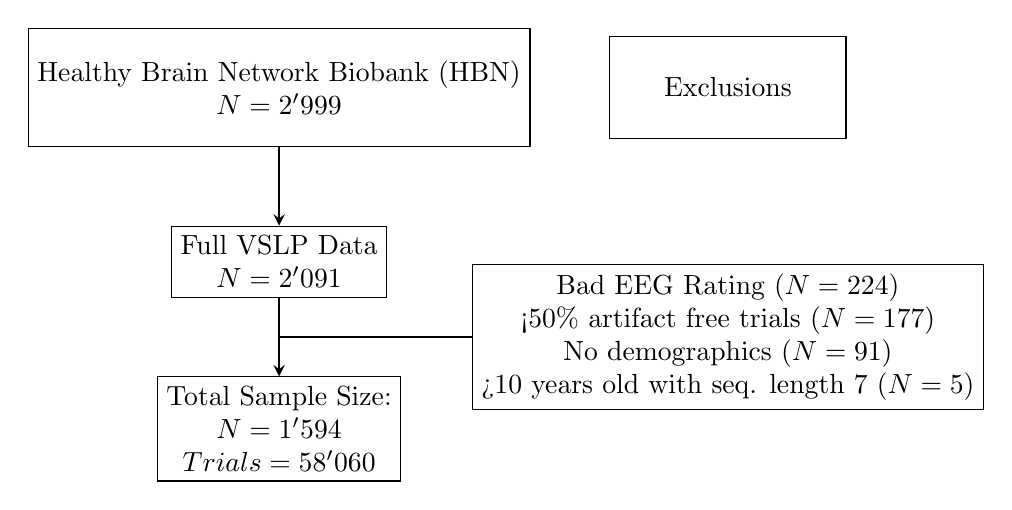
\begin{tikzpicture}%
  [data/.style=
    {draw,minimum height=0.7cm,minimum width=2cm,align=center},
   filter/.style=
    {draw,minimum height=1.3cm,minimum width=3cm,align=center},
   database/.style=
    {draw,minimum height=1.5cm,minimum width=3cm,align=center},
   flow/.style={thick,-stealth},
   apply/.style={}
  ]
  \node[database] (db) {Healthy Brain Network Biobank (HBN)\\$N = 2'999$};
  \node[data,below=of db] (d1) {Full VSLP Data \\ $N=2'091$};
  \node[data,below=of d1] (d2) {Total Sample Size:\\$N=1'594$\\$Trials = 58'060$};
  \draw[flow] (db) -- (d1);
  \draw[flow] (d1) -- coordinate(d1d2) (d2);
  \node[filter,right=of db] (excl) {Exclusions};
  \node[filter] (f1) at (d1d2-|excl) {Bad EEG Rating ($N=224$)\\
                                    <50\% artifact free trials ($N=177$)\\
                                    No demographics ($N = 91$)\\
                                    >10 years old with seq. length 7 ($N=5$)};
  \draw[apply] (d1d2) -- (f1);

\end{tikzpicture}
\caption{Sample Size and Exclusion Criteria.} \label{fig:Diagram}
\end{figure}


\subsection{Visual Sequence Learning Paradigm} \label{VSLP}
The visual sequence learning paradigm (VSLP) \parencite{moiselloNeuralActivationsVisual2013} was one of many tasks applied in the HBN study \parencite[see][]{alexanderOpenResourceTransdiagnostic2017}. During VSLP neurophysiological measures were simultaneously recored, which together with behavioral task performance provided the main data for this thesis.   
In the VSLP participants had to learn a fixed sequence of visual stimulus positions presented one by one. The possible locations were constantly marked by circular outlines with the target stimuli (i.e., to be learned locations) being filled white circles. These possible locations lay equidistant around a ring of fixed eccentricity. The target stimuli appeared for 200 ms each with 1300 ms between them (i.e. inter-stimulus interval). During the presentation, participants were asked to fixate on a central fixation point. To account for floor effects, the length of the sequence was shorter, and the number of possible locations was less for most participants under nine years. Specifically, this meant a sequence of 8 target stimuli with 6 possible locations. For older participants, the sequence consisted of 10 target stimuli and 8 possible locations.  In total, the same sequence was presented five times. After each sequence presentation, participants were asked to recall the locations in a test phase by clicking on them with a computer mouse. The test phase had no time restriction and no feedback was given, whether the correct locations were recalled \parencite{langerResourceAssessingInformation2017}.
Multiple studies with an interest in memory formation and learning processes have applied VSLP \parencite[e.g.,][]{steinemannTrackingNeuralCorrelates2016,strzelczykNeurophysiologicalMarkersSuccessful2022}. Repeated presentation of the same sequence enables the ability to observe learning progress during the recall or test phase. Since VSLP uses highly simplified stimuli, the factors that could influence learning success are minimized \parencite{steinemannTrackingNeuralCorrelates2016}. 

\subsection{Behavioral Data}
Individual target stimuli during each sequence presentation were categorized based on the response of the participants in the test phase. 
Newly learned category (NL) was assigned when the location of the target stimulus was correctly recalled for the first time. Known (K) categorized target stimuli that were correctly recalled at least two consecutive sequence repetitions. Unknown category (UN) classified target stimuli that were not recalled correctly. Finally, the forgotten category (F) was assigned to target stimuli that were NL or K in previous sequence repetitions, and an incorrect recall was made in the current repetition. If a forgotten target stimulus was correctly recalled in a subsequent presentation, the category would change from F to NL. If in a subsequent presentation, a previous forgotten target stimulus is recalled incorrectly again, it becomes unknown. On average, the forgotten category is assigned 9.7\% per participant (see table \ref{tab:avgTLS}).
Furthermore, for every sequence presentation, a knowledge index (KI) was calculated to track the progress of cumulative knowledge of the sequence. The KI was calculated for each sequence presentation of a given participant and was defined as: 
\begin{equation}\label{eq:KI}
    \textrm{Knowledge Index}_{(P,sr)} = \frac{nK_{(P,sr)}+nNL_{(P,sr)}}{nT_{(P,sr)}}
\end{equation}


where P is participant, sr is sequence repetition, K is known category, NL is newly learned and T is the total artifact free trials (see \ref{EEGdatapre}). The KI differed from the one used in \textcite{steinemannTrackingNeuralCorrelates2016} since the paradigm was slightly changed (see \nameref{SuppM}).
Another behavior performance measure used was the learning index (LI). LI is the proportion of newly learned stimuli in a sequence repetition for a given participant and was defined as a ratio of NL stimuli to the total number of stimuli (again only considering artifact free trials): 
\begin{equation} \label{eq:LI}
    \textrm{Learning Index}_{(P,sr)} = \frac{nNL_{(P,sr)}}{nT_{(P,sr)}}
\end{equation}


\subsection{EEG Data Acquisition}
The HBN study, described in \textcite{alexanderOpenResourceTransdiagnostic2017}, used a 128-channel EEG geodesic hydrocel system by Electrical Geodesic Inc. (EGI) with a sampling rate of 500 Hz to record the EEG data. Cz (vertex of the head) was the recording reference and the impedance of each electrode was kept below 40 kOhm. 

\subsection{EEG Data Preprocessing} \label{EEGdatapre}
Since the EEG data was provided in raw format by HBN, the data had to be prepared for further analysis. Data preprocessing was performed using Automagic 2.6, a MATLAB based toolbox for reliable and objective preprocessing in an automatic way \parencite{pedroniAutomagicStandardizedPreprocessing2019}.
Automagic used the PREP pipeline for large-scale EEG analysis \parencite{bigdely-shamloPREPPipelineStandardized2015} to detect noisy or outlier channels. Four criteria are used for detection: extreme amplitudes (deviation exceeding a z-score of 5.00), low correlation with any other channel (correlational threshold: 0.4), lack of predictability by other channels, and unusual high frequency noise (deviation of signal-to-noise ratio exceeding a z-score of 5.00). More detailed descriptions of these processes can be found in \textcite{pedroniAutomagicStandardizedPreprocessing2019} and \textcite{bigdely-shamloPREPPipelineStandardized2015}. Next, automagic handled sweating and power line artifacts by performing a high-pass filter (0.05 Hz) using $pop\_eegfiltnew$ from EEGLAB \parencite{widmannFilterEffectsFilter2012} and a zapline filter (50.00 Hz) using $nt\_zapline$ \parencite[NoiseTools,]{decheveigneZapLineSimpleEffective2020}. Further artifacts caused by, for example, muscle movement were identified and removed using Independent component Label (ICLabel) \parencite{pion-tonachiniICLabelAutomatedElectroencephalographic2019}. 


Following automagic preprocessing procedures, a 45 Hz low-pass filter was applied using $pop\_eegfiltnew$ because only ERP signals are of interest and are mainly below 30 Hz \parencite{luckIntroductionEventrelatedPotential2014}. Next, EEG data was re-referenced to the average of all electrode sites with the $pop\_reref$ function of EEGLAB. Using the average as a reference instead of a single electrode site minimizes artifacts linked to that specific electrode site \parencite{dienIssuesApplicationAverage1998}.
In a second step, the EEG signal was segmented into trials using triggers that marked the appearance of target stimuli (i.e., stimulus onset). The duration of segments was 900 ms (100 pre stimulus onset to 800 ms post stimulus onset). 
At this point two data sets were created, one for visualization purpose and a second data set used to extract P300 amplitudes for statistical analysis. For the first data set, the segmented EEG signals were corrected for baseline using the $pop\_rmbase$ function and a time window of 100 ms pre stimulus onset. The segments of each electrode were compared to an amplitude threshold of -+ 90 microvolts to mark further artifacts. If at any point during a segment this threshold was exceeded, then the trial is marked as artifact and was removed from both data sets. Second, participants who had more than 50\% of their total trials marked as artifacts were excluded from both data sets (see figure \ref{fig:Diagram}). The cutoff point of 50\% was chosen because having a higher cutoff point, for example 75\% would have led to over 1'000 subjects being excluded. 
For the second data set (used for P300 amplitude extraction), the EEG segments of a cluster of centro-parietal electrodes were averaged together, while discarding EEG segments from other electrodes. This cluster consisted of the following electrodes: E54, E55, E61, E62, E78, E79 located at the centro-parietal area. 
Additionally, in this data set no baseline correction was applied. Rather, baseline was included in linear mixed effects models, following the approach of allowing the amount of baseline correction to be determined by statistical model as suggested by \textcite{aldayHowMuchBaseline2019}.


\subsection{Electrode Sites Selection}
The same electrode cluster was selected as in a previous study that used the same paradigm in young and old adults \parencite{strzelczykNeurophysiologicalMarkersSuccessful2022}. In a subsequent step, the grand average scalp topographies of all trials between 150 and 550 ms with a 50 ms step were plotted for different age groups (see figure \ref{fig:elecsel} in \nameref{SuppM}). By visual inspection of these plots, the electrode cluster was considered appropriate in capturing the P300 amplitude for all age groups. Averaging the signal from an electrode cluster where ERP effects are expected has been discussed as a temporary solution to possible differences in the scalp distribution of ERP in young children \parencite{brookerConductingEventRelatedPotential2020}.

\subsection{P300 Extraction}
To extract the P300 amplitude, participants were grouped by age into six bins of two years with the exception of participants 17 years and older, which formed a seventh group with a bin size of 5 years. Reasoning behind the seventh group was to decrease the signal-to-noise ratio, as there were fewer participants in this age range. A time window used to calculate the P300 amplitude was defined by averaging all trials in each age group, resulting in seven grand average ERP waveforms. Using all trials to select the time window (i.e., collapsed localizers) minimizes biases, since differences in conditions are not driving the selection of the time window \parencite{luckIntroductionEventrelatedPotential2014,luckHowGetStatistically2017}. The P300 peak was defined as the most positive amplitude in the time range typical for P300 (i.e., 300 - 500 ms post stimuli onset). Using the latency of the defined peak, a time window was calculated by adding and subtracting 50 ms. In a next step, these time windows were used to calculate the P300 amplitude in each single trial by averaging the voltage in the age appropriate time window (i.e., mean amplitude). Using mean amplitude helps against peak distortion or bias caused by signal noise \parencite{luckIntroductionEventrelatedPotential2014}.

\subsection{Conceptual Replication}
The first part of this thesis aimed at conceptually replicating findings from \textcite{steinemannTrackingNeuralCorrelates2016} and \textcite{strzelczykNeurophysiologicalMarkersSuccessful2022} . A conceptual replication is described as an attempt to test a fundamental idea or hypothesis behind the original study, but can vary in aspects such as experimental operationalization and design, independent and dependent variables and sample population \parencite{crandallScientificSuperiorityConceptual2016}. One main difference from the studies mentioned above was the different sample population. Whereas \textcite{steinemannTrackingNeuralCorrelates2016} investigated neuronal correlates of learning process and memory formation in a sample of healthy young adults and \textcite{strzelczykNeurophysiologicalMarkersSuccessful2022} compared a sample of healthy young adults with healthy old adults, this thesis focused on a sample of children and adolescents with various psychiatric disorders.

\subsubsection{Statistical Analysis}
The main analyses were performed with linear Mixed-Effects Models (LME). LME is a regression-based statistical method that is useful in analyzing hierarchically grouped data \parencite{bickelMultilevelAnalysisApplied2007}.
Event-related potentials are naturally grouped within individuals; therefore, it has often been advocated to apply LME in the analysis of ERP data \parencite{volpert-esmondUsingMultilevelModels2021,vossenMorePotentialStatistical2011}. 
To estimate the models, lme4 package \parencite{batesFittingLinearMixedEffects2015} in R was used with LmerTest \parencite{kuznetsovaLmerTestPackageTests2017} providing p values and the step function used for model selection. The step function follows a data-driven approach of iteratively deleting nonsignificant effects from a specified model. A step-down approach was used, in which the starting point is a full model that is compared to a reduced model using a likelihood-ratio test in an iterative process until the model with the best fit is found. This algorithmic process first determines the structure of random effects and proceeds with the structure of fixed effects \parencite{kuznetsovaLmerTestPackageTests2017}. Specifying the model as input for the step function was done by keeping the fixed effects structure as general as possible (i.e., allowing most fixed effects to interact with each other) and keeping the random part of the model parsimonious since having many random effects led to converging problems during model selection. The model formulas are expressed using the Wilkinson notation \parencite{wilkinsonSymbolicDescriptionFactorial1973}.

\subsubsection{Behavioral Analysis} \label{sec:Behavrioalana}
First, learning performance was analyzed descriptively by plotting behavioral measures (i.e., KI: \ref{eq:KI} and LI: \ref{eq:LI}) over repetitions. More specifically, the group averages of KI and LI with their standard errors were plotted across repetitions to display learning effects and potential age effects. Next, two LME (\ref{eq:mKI}) were specified with KI and LI as dependent variables (continuous: 0-1), repetition (ordinal: 0-4), age (continuous: grand mean centered) and sequence length (categorical: 7 and 10, 10 as reference category) as independent variables. The random effects structure consisted of a random intercept for every participant and a random slope for repetition including their correlation. To help with interpretation of interaction effects as well as having a meaningful intercept, the variables repetition and age were linearly transformed: repetition was subtracted by one, age was mean centered. Therefore, the intercept represented the first repetition and age equal to zero represents an average-aged person. This becomes important for the interpretation of the main effects of explanatory variables that have a significant interaction with age or repetition as these main effects should be interpreted together with the interaction as a system \parencite{hoxMultilevelAnalysisTechniques2017}. Overall, linear transformation does not change the model fit and residuals, and so models with or without linear transformation are equivalent only differing in what part of the model is emphasized \parencite{hoxMultilevelAnalysisTechniques2017}. On the other hand, the random variance of the intercept can be influenced by transformation when a random slope is included in the model \parencite{hoxMultilevelAnalysisTechniques2017}. 

\begin{equation}\label{eq:mKI}
KI \textrm{ or } LI   \sim  Repetition*Age*SequenceLength + (1+Repetition | Participant)
\end{equation}

\subsubsection{Neurophysiological Analysis}
\paragraph{P300 Amplitude Over Sequence Repetitions}
In the context of VSLP, the assumption was that learning a sequence increases its expectancy. As it is suggested that the P300 amplitude decreases as a function of expectancy, changes of P300 amplitude over repetition were analyzed. More specifically, it was hypothesized that over the course of leraning, P300 amplitude decreases. This hypothesis was approached through plots and LME. In the first step, the average P300 amplitude per sequence repetition was calculated for each participant (i.e., mP300). Second, to visualize possible age effects, mP300 was averaged within each age group and plotted across repetitions with error bars reflecting standard errors. Next, a linear mixed effects model was specified (\ref{eq:mP300}) as input for the step function. The specification was as follows: mP300 as dependent variable (continuous: 0-1), repetition (ordinal: 0-4), gender (categorical: male and female, with male as reference category), age (continuous: grand mean centered), sequence length (categorical: 7 and 10, 10 as reference category) and mBase (continuous) as independent variables. mBase was computed by averaging the baseline values of the trials in a given repetition. For every participant, a random intercept was included. 
\begin{equation}\label{eq:mP300}
mP300 \sim Repetition*Age*Gender*SequenceLength + mBase + (1| Participant)
\end{equation}

\paragraph{Predicting Successful Learning}
To further test the possible connection between P300 amplitude and knowledge index, a LME was specified (\ref{eq:mPre}) to investigate whether the differences in KI are explained through differences in mean P300 amplitude. The model was specified with KI as dependent variable (continuous: 0-1), mP300 (continuous), age (continuous: grand mean centered), gender (categorical: male and female, with male as reference category) and mBase (continuous) as independent variables. The model included an intercept as a random effect.

\begin{equation}\label{eq:mPre}
KI \sim mP300*Age*Gender +  mBase + (1 | Participant)
\end{equation}

\paragraph{P300 Amplitude Across Learning Categories}
In a final step, differences in P300 amplitude across learning categories (i.e., Unknown, Newly Learned, Known, Forgotten) were analyzed to directly tie the amplitude of P300 to the behavioral response at a single trial level. Since learning categories differentiate between first accurate recall of a spatial location (i.e., Newly Learned) and subsequent accurate recall (i.e., Known), these categories provide additional information which can be used to refer to how well a spatial location is learned or to what degree it is expected. Connecting P300 amplitude to learning categories on a single trial level is important, as only analyzing the P300 amplitude as an average of a sequence repetition can be influenced by habituation \parencite{ravdenHabituationP300Visual1998}. 
Topographical plots were created for the learning categories Unknown, Newly Learned and Known for four randomly selected age groups. For visualization, baseline corrected data set was used and all trials of each learning category were averaged together. Potential age effects were checked by plotting the average P300 amplitude and ERP's of learning categories across age groups the same age groups. In a next step, a LME model was specified (\ref{eq:mCat}). The model consisted of P300 as dependent variable, learning categories (categorical: UN,NL,K,F with NL as reference category), age, gender and base as independent variables, and a random intercept for each participant.  
\begin{equation}\label{eq:mCat}
P300 \sim LearningCategories*Age*Gender + base + (1 | Participant)
\end{equation}
Since LME only compares each learning category to the reference category, contrasts between the learning categories were computed using the emmeans package in R Studio while correcting for multiple comparisons using Bonferroni correction \parencite{lenthPackageEmmeans2019}. 

\subsection{Exploratory Analysis}
The second part of the thesis explored whether successful learning in VSLP and the degree of decrease in the amplitude of P300 over repetitions are associated with transdiagnostic constructs related to learning. 

\subsubsection{Knowledge Index and P300 Decrease}
For every participant, an average of their repetition based knowledge index was calculated.  
Second, a measurement reflecting the degree of a participants increase in expectancy of sequence was created. For this, a linear regression with P300 amplitude as dependent variable and repetition as independent variable was specified for each participant. The resulting slope coefficient of repetition was used in the exploratory part. 

\subsubsection{Questionnaires and Tests}
Since this part is exploratory in nature, no theoretical framework guided the inclusion of questionnaires. Instead, questionnaires that were filled out by most participants were considered and subscales of these questionnaires that have been found to be relevant for either learning, working memory test performance, or P300 amplitude were included. If available, standardized scores were used; otherwise, raw scores were included.

\subsubsection{SWAN}
The Strengths and Weaknesses of ADHD symptoms and Normal behavior scale \parencite[SWAN][]{swansonGenesAttentiondeficitHyperactivity2001}) provided scores for attention problems. SWAN has a bidirectional questionnaire design assessing problems but also strength of symptoms relevant in ADHD with a 7-point scale with endpoints: far below average and far above average \parencite{alexanderMeasuringStrengthsWeaknesses2020}. This questionnaire has been applied in multiple areas such as genetic studies, pharmacotherapeutics, neuropsychology, and has been shown to have good psychometric properties \parencite[for review see][]{britesDevelopmentApplicationsSWAN2015}. 
Of interest in this thesis was the subscale inattention, as impaired attention has been reported as one of the most ubiquitous clinical symptoms \parencite{mirskyNosologyDisordersAttention2001} and plays an important role in maintaining relevant information \parencite{chunVisualWorkingMemory2011}. Therefore, the scores of the inattention subscale were included in the analysis (i.e., raw scores). 

\subsubsection{WISC-V}
Scores from the fifth edition Wechsler intelligence scale for children \parencite[WISC-V][]{wechslerWechslerIntelligenceScale2014} were included in the exploratory analysis. More specifically, two primary index scores (i.e., processing speed index and working memory index). For psychometric properties and a more detailed review of this test, see \textcite{wechslerWechslerIntelligenceScale2014} and \textcite{meyerScoresSpaceMultidimensional2018}. Working memory has been stated as an important factor in learning and memory \parencite{cowanWorkingMemoryUnderpins2014} and is prominently associated with P300 in the theoretical framework of context updating \parencite{donchinP300ComponentManifestation1988,lenartowiczUpdatingContextWorking2010}. Therefore, working memory index was included in the exploratory analysis. Processing speed index as second variable was included since it has been shown to be affected in multiple psychiatric disorders and is linked to academic performance \parencite{mayesLearningAttentionWriting2007}.

\subsubsection{Conners 3}
Subscale Learning Problems of the Conners 3 self report \parencite{connersConners2008} was used to explore whether behavioral or neurophysiological measures of learning are associated with learning problems. The psychometric properties of Conners 3 have been reported to be good \parencite{connersConners2008}.

\subsubsection{Child Behavior Checklist}
Five subscales were included from the parent report version of the Child Behavior Checklist questionnaire (CBCL) \parencite{achenbachManualChildBehavior1991}. More specifically, standard scores of the subscales Withdrawn/Depressed, Rule Breaking Behavior, Attention Problems, Anxious/Depressed, and Aggressive Behavior were included. Following an approach done in previous studies, the latter three subscales (i.e., Attention Problems, Anxious/Depressed, Aggressive Behavior) were summed together to arrive at an index for deficits in emotional regulation: CBCL-AAA profile \parencite{biedermanSeverityAggressionAnxietydepression2012,donfrancescoDeficientEmotionalSelfRegulation2015}. Emotional dysregulation has been stated as a main transdiagnostic construct affecting multiple disorders \parencite{sloanEmotionRegulationTransdiagnostic2017} and was therefore included to explore its effect on knowledge index and P300 amplitude decrease.

\subsubsection{Social Responsiveness Scale}
The subscales Social Motivation Problems and Social Cognitions of the Social Responsiveness Scale \parencite{wighamReliabilityValiditySocial2012} were included in the exploratory analysis. The validity and reliability of this questionnaire have been reported to be good \parencite{wighamReliabilityValiditySocial2012}. Including these variables followed the notion that, especially in school settings, social aspects can influence learning and performance \parencite{wentzelAcademicSocialMotivational1998a}.

\subsubsection{Network Analysis}
Altered P300 has been associated with many psychiatric disorders \parencite{polichClinicalApplicationP3002004,surEventrelatedPotentialOverview2009} and seems to reflect a general vulnerability \parencite{surEventrelatedPotentialOverview2009} rather than related to a particular disorder \parencite{duncanEventrelatedPotentialsClinical2009}. Often the findings of altered P300 are mixed when investigating a single disorder \parencite{salgariEventrelatedPotentialsRare2021}. Additionally, P300 has been shown to be sensitive to cognitive dysfunction \parencite{polichCognitiveBiologicalDeterminants1995,potterAssessmentMildHead1999} which itself has been discussed as a transdiagnostic phenomenon in psychopathology moderated by factors such as motivation or emotion \parencite{abramovitchFactorCognitiveDysfunction2021}. This suggests that it may be of importance to study P300 in a transdiagnostic manner. 
Recently, network analysis has been shown to be a promising tool in studying transdiagnostic phenomena \parencite[e.g.,][]{astleAnnualResearchReview2022,borsboomReflectionsEmergingNew2022,chavez-baldiniRelationshipCognitiveFunctioning2021}. 

To explore the question whether the selected transdiagnostic variables provide information on behavioral (i.e., Knowledge Index) and neurophysiological (i.e., P300 decrease) measures obtained from the visual sequence learning paradigm, a network model was estimated. 
As described in \textcite{isvoranuNetworkPsychometricsGuide2022}, network models are statistical structures 
with nodes (i.e., variables) and connecting edges (i.e., estimated statistical relations). Most often these statistical relations are estimated with partial correlations in an undirected manner using Pairwise Markov Random Fields models (PMRFs). In PMRFs the absence of a connection (i.e., edge) between two nodes indicates that these variables are conditional independent after controlling for all other variables (i.e., parietal correlation). The presence of an edge reflects a conditional dependency, with the partial correlation coefficient being the strength of this relationship. A subclass of PMRF models used in this analysis is the Gaussian graphical model \parencite[GGM,][]{lauritzenGraphicalModels1996} which is used when the variables in the network (i.e., nodes) are continuous.
With PMRFs, the predictive relationships between variables in a network model are visualized and would be comparable to computing many exploratory regression analyses \parencite{isvoranuNetworkPsychometricsGuide2022}.  

\paragraph{Procedure}
In a first step, selected variables were plotted to inspect their distribution (see figure \ref{fig:distall} in \nameref{SuppM}). Three highly skewed variables (i.e., subscales from CBCL) were transformed with a nonparanormal transformation \parencite{liuNonparanormalSemiparametricEstimation2009} using the function $huge.npn$ from the huge package \parencite{zhaoHugePackageHighdimensional2012}. This transformation approach uses the cumulative distribution of the data and maps each point to a z-value of a standard normal distribution via the cumulative distribution of the standard normal distribution \parencite{liuNonparanormalSemiparametricEstimation2009}. The estimate of the model was made using the $estimateNetwork$ function of the bootnet package \parencite{epskampPackageBootnet2015}. There are different estimation (and model selection) methods that come with the bootnet package, and the $ggmModSelect$ method was chosen for this analysis. Different estimation methods can produce different results. At this point, however, no clear method is to be preferred and one has to consider the research question and sample size while choosing the estimation method \parencite{isvoranuWhichEstimationMethod2021}. Although it has been observed through simulation studies that with a medium sample size (e.g., N = 1000), $ggmModSelect$ produces estimates with good specificity (i.e., proportion of true absent edges selected in the estimated network) and sensitivity (i.e., proportion of true edges selected in the estimated network) in detecting edges that connect different domains in the network structure (i.e., bridge edges).  
The algorithmic approach of $ggmModSelect$ is described in \textcite{isvoranuNetworkPsychometricsGuide2022}. First, to limit the search space for the model, $ggmModSelect$ estimates various partial correlation matrices with different regularization parameters \footnote{optimizing likelihood function while penalizing for model complexity to a varying degree \parencite{isvoranuNetworkPsychometricsGuide2022}} using glasso \parencite{friedmanSparseInverseCovariance2008}. Next, the resulting models are re-estimated without using regularization and the model structure with the lowest Bayesian information criterion (BIC) is selected. Edges in the selected model are included or removed in an iterative process to once again minizime BIC \parencite{isvoranuNetworkPsychometricsGuide2022}.   
The final model consisted of a partial correlation matrix that was then visualized using the qgraph package \parencite{epskampQgraphNetworkVisualizations2012}. Lastly, the accuracy of edges were estimated using bootstrapped confidence intervals. This was accomplished with non-parametric bootstrapping (bootnet package) in which observations are resampled with replacement and results in 1000 new data sets. When using unregularized estimates of edges (e.g., ggmModSelect), the bootstrapped confidence intervals are reported to be valid as null hypothesis tests \parencite{epskampEstimatingPsychologicalNetworks2018}.


\clearpage

\section{Results}\label{Results}
\subsection{Behavioral Results}
\subsubsection{Demographics}
The basic demographics of the sample are displayed in table \ref{tab:demo}.
\begin{table}[H]
\centering
    \begin{tabular}{llllllll}
    \hline

    \multicolumn{2}{c}{\textbf{N}} & \multicolumn{4}{c}{\textbf{Age}}                                                                                                        & \multicolumn{2}{c}{\textbf{Gender}}                                \\ \hline
                    &          & \multicolumn{1}{c}{\textbf{Mean}} & \multicolumn{1}{c}{\textbf{SD}} & \multicolumn{1}{c}{\textbf{Min}} & \multicolumn{1}{c}{\textbf{Max}} & \multicolumn{1}{c}{\textbf{M/F}} & \multicolumn{1}{c}{\textbf{\%}} \\ \cline{3-8}
\textbf{SL7}         & 541      & 7.39                              & 0.99                            & 5.04                             & 9.93                             & 390/151                          & 72/28                           \\
\textbf{SL10}        & 1'053     & 12.50                             & 2.92                            & 8.15                             & 21.90                            & 762/291                          & 72/28                           \\
\textbf{Total}      & 1'594     & 10.77                             & 3.44                            & 5.04                             & 21.90                            & 1'152/442                         & 72/28    \\ \hline     
 \multicolumn{8}{l}{\small \textit{Note.} SL7 = Sequence Length 7. SL10 = Sequence Length 10.}
\end{tabular}
\caption{Basic Demographics}
    \label{tab:demo}
\end{table}

\subsubsection{Diagnoses}
To broadly characterize the sample, table \ref{tab:diag} shows the number of participants who received no diagnosis, a single diagnosis and those participants with multiple diagnoses. Furthermore, the most frequent diagnoses are displayed. 
\begin{table}[H]
\centering
\begin{tabular}{lc}
\hline
\textbf{General}                  & \textbf{N}       \\ \hline
No Diagnosis                      & 158              \\
One Diagnosis                     & 644              \\
Comorbidity                       & 793              \\ \hline
\multicolumn{2}{l}{\textbf{Most Frequent Diagnoses}} \\ \hline
Attention-Deficit/Hyperactivity Disorder                              & 902              \\
Anxiety Disorder                  & 517              \\
Specific Learning Disorder        & 331              \\
Autism Spectrum Disorder          & 251              \\ \hline
\end{tabular}
\caption{Most Frequent Diagnoses}
    \label{tab:diag}
\end{table}

\subsubsection{Visual Sequence Learning Task Performance}
As depicted in table \ref{tab:avgTLS}, participants that learned the shorter sequence had on average 27.42 (4.61) artificial free trials, while participants assigned to the longer sequence had on average 41.05 (6.95) artificial free trials. Across sequence repetitions, participants with SL7 had on average 11.58 (6.02) trials categorized as unknown, 6.04 (2.35) as newly learned, 7.06 (6.03) as known, and 2.74 (1.85) as forgotten. A similar pattern was found in participants with SL10 where, on average, the highest proportion of trials was categorized as unknown followed by known and newly learned. 
\begin{table}[H]
\centering
\begin{tabular}{lccccc}
\hline

\multicolumn{2}{c}{\textbf{Trials}}                & \multicolumn{4}{c}{\textbf{Learning Categories}}                     \\ \hline
            &   & \textbf{UN} & \textbf{NL} & \textbf{K} & \textbf{F} \\ \cline{3-6} 
\textbf{SL7}    & 27.42 (4.61)                              & 11.58 (6.02)      & 6.04 (2.35)       & 7.06 (6.03)      & 2.74 (1.85)     \\
&&43.03 \% & 22.00 \% &25.01 \%&9.96 \%\\
\textbf{SL10}   & 41.05 (6.95)                               & 18.08 (8.90)      & 8.80 (3.28)       & 10.26 (8.54)     & 3.93 (2.60)      \\
&& 44.69 \% & 21.40 \% & 24.30 \% & 9.61 \% \\
\textbf{Total} & 36.42 (8.99)                              & 15.87 (8.61)      & 7.86 (3.26)     & 9.17 (7.92)     & 3.52 (2.43)      \\
&& 44.13 \% &21.61 \% &24.54 \% & 9.73 \% \\\hline 
\multicolumn{6}{l}{\small \textit{Note.} UN = Unknown, NL = Newly Learned, K = Known, F = Forgotten.}\\[-0.3cm]
\multicolumn{6}{l}{\small Average Trials and Learning Categories per participant with standard deviation.}
\end{tabular}
\caption{Average Trials and Learning Categories per Participant}
\label{tab:avgTLS}
\end{table}







\paragraph{Knowledge Index}
It was hypothesized that behavioral performance increases over the course of learning and that this performance increases with age during childhood and adolescents. To test these hypotheses, first behavioral measures KI and LI were plotted over repetitions for each age group. Second, linear mixed-effects models were fitted for inferential testing. 
Figure \ref{fig:KI_LI} shows the average knowledge and learning index across repetitions for each age group (error bars are standard errors). Plotting KI over repetitions suggested that, on average, behavioral performance (i.e., KI) increased over repetitions and that older participants had higher behavioral performance (i.e., KI). The average learning index was highest in the first repetition, with no obvious age differences visible. 
\begin{figure}[H]
    \centering
    \includesvg[width=\textwidth]{Figures/KI_LI_rep}   
    \caption{Knowledge Index and Learning Index over Repetitions}
    \label{fig:KI_LI}
\end{figure}

Providing inferential evidence was provided with a linear mixed effects model (results in table \ref{tab:ReKI}). The best-fit model of knowledge index (\ref{eq:mKI2}) had a fixed effects structure consisting of repetition (REP), age, sequence length (SL) and three interactions. Random effects structure included random intercept for participant, a random slope for repetition and their correlation: 
\begin{equation}\label{eq:mKI2}
KI \sim REP + Age + SL + REP\,x\,SL + REP\,x\,Age + Age\,x\,SL + (1+REP | Participant)
\end{equation}
As mentioned in the section \nameref{sec:Behavrioalana}, variables age and repetition were linearly transformed to help with interpretation of interaction \parencite{hoxMultilevelAnalysisTechniques2017}. Therefore, in the resulting model, the intercept reflected the average KI for average aged participants with a sequence length of 10 in the first repetition (i.e., expected KI when all explanatory variables are zero). Because a random slope (i.e., repetition) was included, the estimated variance of the intercepts was influenced by the linear transformation and thus reflected the variance of intercepts for average aged participants with SL10 in first repetition (i.e., conditioned on all explanatory variables being equal to zero) \parencite{hoxMultilevelAnalysisTechniques2017}.

A significant main effect of repetition ($\beta$  = 0.033, CI = [0.03 ; 0.04], p <0.001) indicated that for participants of average age with a sequence length (SL) of 10, KI increased with repeated presentation of sequence. This increase was moderate by age ($\beta$  = 0.005, CI = [0.003;0.006], p <0.001) and SL ($\beta$  = 0.016, CI = [0.005;0.028], p = 0.006). Therefore, the model suggested that the effect of repetition on KI increased with age. Moderation of sequence length on the effect of repetition suggested that, for participants of average age, the effect of repetition on KI is greater in SL7 compared to SL10. This moderation should be interpreted with caution since no actual data is observed at this described age point (i.e., there are no participants of average age who had an SL of 7). Second, age significantly explained the differences in KI in the first repetition suggested by a main effect of age ($\beta$  = 0.015, CI = [0.01; 0.02], p<0.001). This indicated that KI in the first repetition was higher in older participants. The effect of age on KI in the first repetition was stronger in participants with sequence length 7 as suggested by a significant interaction of age and sequence length 7 ($\beta$ = 0.016, CI =  [0.005; 0.028], p = 0.006). Random components of the model revealed a large variance in effect of repetition. Exploring the random slopes estimated by lmer, revealed that 868 participants had a negative slope.  

Taken together, the model suggests that participants increase their knowledge of the sequence over repetitions. Additionally, age effects are revealed by the model with older participants having an increased effect of repetition on KI. A second age effect suggested by the model is that KI in the first repetition is on average higher for older participants. 


\begin{table}[H]
\centering
\begin{tabular}{lccccc}
\hline
\textbf{Variable}            & \textbf{Beta} & \textbf{SE}          & \textbf{CI}           & \textbf{t-value} & \textbf{p-value} \\ \hline
Intercept                    & 0.363         & 0.007                & 0.35 - 0.38           & 50.08            & \textless{}0.001 \\
Rep                          & 0.033         & 0.003                & 0.03 - 0.04           & 12.83            & \textless{}0.001 \\
Age                          & 0.015         & 0.002                & 0.01 - 0.02           & 6.67             & \textless{}0.001 \\
SL (7)                       & 0.291         & 0.037                & 0.22 - 0.36           & 7.90             & \textless{}0.001 \\
Rep x Age                    & 0.005         & 0.001                & 0.003 - 0.006         & 5.75             & \textless{}0.001 \\
Rep x SL (7)                 & 0.016         & 0.006                & 0.005 - 0.028         & 2.76             & 0.006            \\
Age x SL (7)                 & 0.048         & 0.009                & 0.03 - 0.07           & 5.23             & \textless{}0.001 \\ \hline
\textbf{Variance Components} & \textbf{SD}   & \multicolumn{2}{l}{\textbf{Goodness of fit}} & \textbf{}        & \textbf{}        \\ \hline
Participant                  & 0.14          & \multicolumn{2}{l}{Log Likelihood}           & -461.09          &                  \\
Rep                          & 0.04          &                      &                       &                  &                  \\
Cor(Participant, Rep)        & 0.53          &                      &                       &                  &                  \\
Residual                     & 0.21          &                      &                       &                  &                  \\ \hline
\multicolumn{6}{l}{\small \textit{Note.} Rep = Repetition, SL7 = Sequence Length 7, SL10 = Sequence Length 10.}\\[-0.3cm]
\multicolumn{6}{l}{\small Intercept represents average aged participants with SL10 at first repetition.}\\
\end{tabular}
\caption{Model Output: Increase in Knowledge Index over Repetitions}
\label{tab:ReKI}
\end{table}

%%%%%%%%%%%%%%%%%%%%%%%%%%%%%%%%%%%%%%%%%%%%%%%%%%%%%%%%%%%%%%%%%
%%%%%%%%%%%%%%%%%%%%%%%%%%%%%%%%%%%%%%%%%%%%%%%%%%%%%%%%%%%%%%%%%

\paragraph{Learning Index}
Learning Index was a second behavioral index of learning and is mentioned here for the sake of completeness even though it was not a focus in this thesis.
For the learning index, no random effect structure could be estimated. Therefore, the best-fit model was a linear multiple regression model (\ref{eq:mLI}) and results are displayed in table \ref{tab:ReLI}).

\begin{equation}\label{eq:mLI}
LI \sim REP + Age + SL + REP\,x\,Age + REP\,x\,SL + Age\,x\,SL + REP\,x\,Age\,x\,SL
\end{equation}

A significant main effect of repetition on learning index was found ($\beta$ = -0.041, CI = [-0.05; -0.04], p<0.001). This suggested that on average the learning index decreased with repetition for participants of average age with sequence length 10 and decreased even further with increasing age ($\beta$ = -0.003, CI = [-0.004; -0.002], p<0.001). The three way interaction of repetition, age, and sequence length 7 suggested that the decreasing effect of age on repetition is even stronger for participants with sequence length 7 ($\beta$ = -0.014, CI = [-0.02; - 0.01], p<0.001). Furthermore, older age was associated with a higher learning index in the first repetition in SL10 ($\beta$= 0.011, CI = [0.01; 0.02], p<0.001) and even more so in participants with SL7 ($\beta$ = 0.031, CI = [0.02; 0.05], p<0.001). 

\begin{table}
\centering
\begin{tabular}{lccccc}
\hline
\textbf{Variable}            & \textbf{Beta} & \textbf{SE}          & \textbf{CI}           & \textbf{t-value} & \textbf{p-value} \\ \hline
Intercept                    & 0.286         & 0.006                & 0.28 - 0.30           & 50.09            & \textless{}0.001 \\
Rep                          & -0.041         & 0.002                & -0.05 - -0.04           & -18.33            & \textless{}0.001 \\
Age                          & 0.011         & 0.002                & 0.01 - 0.02           & 6.41             & \textless{}0.001 \\
SL (7)                       & 0.201         & 0.029                & 0.14 - 0.26           & 6.80             & \textless{}0.001 \\
Rep x Age                    & -0.003         & 0.001                & -0.004 - -0.002         & -4.14             & \textless{}0.001 \\
Rep x SL (7)                 & -0.078         & 0.012                & -0.10 - -0.05         & -6.45             & \textless{}0.010            \\
Age x SL (7)                 & 0.031         & 0.007                & 0.02 - 0.05          & 4.21             & \textless{}0.001 \\ 
(Rep x Age) x SL (7) & -0.014 & 0.003 & -0.02 - -0.01 & -4.56 & \textless{}0.001 \\ \hline
\multicolumn{6}{l}{\small \textit{Note.} Rep = Repetition, SL7 = Sequence Length 7, SL10 = Sequence Length 10.}\\[-0.3cm]
\multicolumn{6}{l}{\small Intercept represents average aged participants with SL10 at first repetition.}\\
\end{tabular}
\caption{Model Output: Decrease in Learning Index over Repetitions}
\label{tab:ReLI}
\end{table}

\subsection{Neurophysiological Results}
Thus far it was shown that the estimated linear mixed effects models suggested that participants on average increase their knowledge of the sequence over the course of learning and that older participants tended to learn greater proporation of the sequence (i.e., KI). In a next step, it was investigated how the neurophysiological measure (i.e., P300 amplitude) changed over the course of learning.
\subsubsection{P300 Amplitude over Repetitions}
Firstly, the mean P300 amplitude in each age group was plotted over sequence repetition (see figure \ref{fig:KI_LI}). This plot gave the first impression that P300 amplitude decreased over repetitions and that there were potential age effects involved. Plotting ERP of repetitions for four randomly selected groups is depicted in figure \ref{fig:erp_rep} and showed the decrease in amplitude around 400 ms across repetitions. 
%plot
\begin{figure}[H]
    \centering  
    \includesvg[width =0.8\textwidth]{Figures/meanP_rep}   
    \caption{Decrease of Mean P300 Amplitude over Repetitions}
    \label{fig:KI_LI}
\end{figure}
%ERP
\begin{figure}[H]
    \centering
    \includesvg[width =\textwidth]{Figures/erp_age_rep_c}   
    \caption{ERP over Repetitions Visualized for Four Groups}
    \label{fig:erp_rep}
\end{figure}

Second, a mixed-effects model was selected by the step function to provide inferential evidence for changes in mean P300 amplitude over repetition. The selected model was: 
\begin{equation}\label{eq:mP3002}
mP300 \sim REP + Age + Gender + SL  + mBase + REP \,x\, Age + REP 
\,x \,SL + (1 | Participant).
\end{equation}


In average aged participants with sequence length 10, mean P300 amplitude decreased significantly on average with repetition ($\beta$ = -0.104, CI = [-0.12; -0.09], p < 0.001). This decrease was significantly stronger in older age ($\beta$ = -0.008, CI = [-0.011; -0.005], p<0.001). However, age did not explain the differences in the mean P300 amplitude in the first repetition ($\beta$ = -0.006, CI = [-0.03; -0.52], p = 0.605). A significant interaction of repetition and sequence length 7 ($\beta$ = -0.091, CI = [-0.12; -0.07], p<0.001) indicated that the effect of repetition is further moderated by SL, meaning that average aged participants in SL7 had a stronger decrease compared to SL10. This interaction should be viewed with caution since no actual data was observed in this range (i.e., no average aged participants had SL of 7). Mean P300 amplitude was significantly higher in the first repetition for participants with sequence length 7 compared to participants with SL10 ($\beta$ = 0.209, CI = [0.04; 0.40], p = 0.017). On average, female participants had lower P300 amplitudes compared to male participants ($\beta$ = -0.162, CI = [-0.29; -0.04], p = 0.010). 
\begin{table}[H]
\centering
\begin{tabular}{lccccc}
\hline
\textbf{Variable}            & \textbf{Beta} & \textbf{SE}          & \textbf{CI}           & \textbf{t-value} & \textbf{p-value} \\ \hline
Intercept                    & 1.166         & 0.042                & 1.08 - 1.25           & 27.63            & \textless{}0.001 \\
Rep                          & -0.104         & 0.005                & -0.12 - -0.09           & -19.077          & \textless{}0.001 \\
Age                          & -0.006         & 0.012                & -0.03 - 0.02           & -0.52             & 0.605 \\
Gender (F)                 &-0.162      & 0.063                & -0.29 - -0.04           & -2.57            & 0.010 \\
SL (7)                       & 0.209         & 0.087                & 0.04 - 0.40           & 2.38             & 0.017 \\
meanBase                 & -0.223         & 0.044                & -0.23 - -0.21           & -49.98             & \textless{}0.001 \\
Rep x Age                    & -0.008         & 0.002                & -0.011 - -0.005         & -5.00             & \textless{}0.001 \\
Rep x SL (7)                 & -0.091         & 0.013                & -0.12 - -0.07         & -6.90             & \textless{}0.001            \\ \hline
\textbf{Variance Components} & \textbf{SD}   & \multicolumn{2}{l}{\textbf{Goodness of fit}} & \textbf{}        & \textbf{}        \\ \hline
Participant                  & 1.10          & \multicolumn{2}{l}{Log Likelihood}           & -106636.4         &                  \\

Residual                     & 1.46          &                      &                       &                  &                  \\ \hline
\multicolumn{6}{l}{\small \textit{Note.} Rep = Repetition, SL7 = Sequence Length 7, SL10 = Sequence Length 10.}\\

\end{tabular}
\caption{Model Output: Decrease in Mean P300 Amplitude over Repetitions}
\label{tab:my_label}
\end{table}
\subsubsection{Predicting Learning Success}
After finding that mean P300 amplitude decreased over repetition, the next step consisted of examining whether the knowledge index could be predicted by mean P300 amplitude of a given sequence repetition within participants. Step function selected the following model as having the best fit (with results in table \ref{tab:predKI}): 
\begin{equation}\label{eq:mPre2}
KI \sim mP300 + Age + Gender +  Age \,x\, Gender + (1 | Participant).
\end{equation}
The model had a fixed effect structure of age, gender, and their interaction and intercept as random effect.
A significant main effect of mean P300 amplitude ($\beta$ = -0.003, CI = [-0.006; -0.001], p = 0.025) revealed by the model suggested that increases in KI are associated with decreases in mean P300 amplitude. Furthermore, the step function selected a model without interaction between mean P300 amplitude and age, suggesting that the predictability of mean P300 amplitude is similar across age. 
\begin{table}[H]
\centering
\begin{tabular}{lccccc}
\hline
\textbf{Variable}            & \textbf{Beta} & \textbf{SE}          & \textbf{CI}           & \textbf{t-value} & \textbf{p-value} \\ \hline
Intercept                    & 0.468         & 0.007                & 0.46 - 0.48           & 67.94            & \textless{}0.001 \\
meanP300                          & -0.003         & 0.001                & -0.006 - -0.001           & -2.25          & 0.025 \\
Age                          & 0.009         & 0.002                & 0.005 - 0.013           & 4.72             & \textless{}0.001  \\
Gender (F)                 &0.014      & 0.013                & -0.01 - 0.04           & 1.12            & 0.264\\
Age x Gender (F)                    & 0.010         & 0.004                & 0.003 - 0.017         & 2.84             & 0.004 \\\hline
\textbf{Variance Components} & \textbf{SD}   & \multicolumn{2}{l}{\textbf{Goodness of fit}} & \textbf{}        & \textbf{}        \\ \hline
Participant                  & 0.20          & \multicolumn{2}{l}{Log Likelihood}           & -106636.4         &                  \\

Residual                     & 0.23          &                      &                       &                  &                  \\ \hline

\end{tabular}
\caption{Model Output: Predicting Differences in KI with Mean P300 Amplitude}
\label{tab:predKI}
\end{table}
\subsubsection{P300 Amplitude and Learning Categories}
So far it was established that on average participants increase their knowledge of sequence over the course of learning and that this was accompanied by a decrease in mean P300 amplitude over repetitions. Furthermore, the KI could be predicted by mean P300 amplitude within participants. Learning categories for individual stimuli differed in P300 amplitude regardless of repetition. The reason for this analysis was two fold. First, to disentangle the possibility that the decrease in P300 amplitude was due to habituation effects. Second, to provide a stronger link to behavioral measures of learning on a stimulus level rather than a sequence level. Plotting the average ERPs of learning categories for four randomly selected age groups (\ref{fig:erp_ls}) indicated that the P300 peaks differ between the learning categories. Furthermore, plotting the topography of the learning categories \ref{fig:topo} indicated that the known stimuli had a lower and more widespread distribution of positive voltage compared to unknown stimuli.
%erp
\begin{figure}[H]
    \centering
    \includesvg[width =\textwidth]{Figures/erp_age_learningstates_c}   
    \caption{ERP of Learning Categories Visualized for Four Groups}
    \label{fig:erp_ls}
\end{figure}


%topo
\begin{figure}[H]
     \centering
     \includesvg[width =\textwidth]{Figures/topolearning}   
    \caption{Topoplots of Learning Categories Visualized for Four Groups}
    \label{fig:topo}
\end{figure}
\newpage
A final mixed effects model was selected with fixed effects structure of LearningCategories (reference: NL), Age, Gender, and base, as well as a random intercept for every participant (results in table \ref{tab:ReP3Cat}):   

\begin{equation}\label{eq:mCat2}
P300 \sim LearningCategories +  Age + Gender + base + (1 | Participant).
\end{equation}

The model revealed the following results.
Learning categories forgotten ($\beta$ = -0.202, CI  =[-0.33; -0.07], p = 0.002) and known ($\beta$ = -0.378, CI = [-0.48; -0.28], p<0.001) had significantly lower P300 amplitudes compared to newly learned, while stimuli categorized as unknown did not differ significantly ($\beta$ = -0.068, CI = [-0.16; -0.02], p = 0.133). Overall, age is associated with lower P300 amplitudes ($\beta$ = -0.024, CI = [-0.04; -0.01], p = 0.003) but the step function did not select an interaction between learning categories and age, suggesting similar differences between newly learned and other learning categories across age. 

\begin{table}[H]
\centering
\begin{tabular}{lccccc}
\hline
\textbf{Variable}            & \textbf{Beta} & \textbf{SE}          & \textbf{CI}           & \textbf{t-value} & \textbf{p-value} \\ \hline
Intercept                    & 1.118         & 0.046                & 1.03 - 1.21           & 24.36           & \textless{}0.001 \\
Forgotten                          & -0.202        & 0.065                & -0.33 - -0.07           & -3.10         & 0.002 \\
Known                          & -0.378         & 0.050               & -0.48 - -0.28           & -7.53            & \textless{}0.001  \\
Unknown                          & -0.068         & 0.045              & -0.16 - -0.02           & -1.50            & 0.133  \\
Age                          & -0.024         & 0.008             & -0.04 - -0.01           & -2.95           & 0.003  \\
Gender (F)                 & -0.155      & 0.062                & -0.28 - -0.03           & -2.52           & 0.012\\
mBase                    & -0.232         & 0.004                & -0.24 - -0.22         & -54.12             & \textless{}0.001 \\\hline
\textbf{Variance Components} & \textbf{SD}   & \multicolumn{2}{l}{\textbf{Goodness of fit}} & \textbf{}        & \textbf{}        \\ \hline
Participant                  & 0.87          & \multicolumn{2}{l}{Log Likelihood}           & -164135.2        &                  \\

Residual                     & 4.03         &                      &                       &                  &                  \\ \hline

\end{tabular}
\caption{Model Output: P300 Amplitude Differences in Learning Categories}
\label{tab:ReP3Cat}
\end{table}


Next, a pairwise post hoc comparison of the learning categories was performed since the mixed effects model only compares each learning category with the reference category. The post hoc comparison was for average aged participants, but since the model did not include an interaction between age and learning categories the differences between learning categories were thought to be comparable across age. As shown in table \ref{tab:posthoc}, known stimuli had significantly lower P300 amplitudes compared to unknown stimuli or forgotten. Furthermore, forgotten stimuli did not differ significantly from unknown stimuli.

\begin{table}
\centering
\begin{tabular}{lccc}
\hline
\textbf{Contrast}            & \textbf{Effect Size} & \textbf{CI}          & \textbf{p-value*}          \\ \hline
NL - K                    & 0.094         & 0.07 - 0.12                &  \textless{}0.001 \\
NL - UN                          & 0.017              & -0.005 - 0.04                  & 0.796 \\
NL - F                          & 0.050         & 0.02 - 0.08                         & 0.012 \\
K - UN                     & -0.077         & -0.10 - -0.05                           & \textless{}0.001 \\
F - K                   & 0.044         & 0.01 - 0.07                       & 0.048 \\
F - UN                 & -0.033                      & -0.06 - -0.004                & 0.164             \\ \hline
\multicolumn{4}{l}{\small \textit{Note}. NL = Newly Learned, K = Known, UN = Unknown, F = Forgotten.}\\[-0.3cm]
\multicolumn{4}{l}{\small *Bonferroni corrected.}\\
\end{tabular}
\caption{Post Hoc Contrasts of Learning Categories}
\label{tab:posthoc}
\end{table}
\subsection{Exploratory Analysis}

Using $ggmModSelect$ the final model structure arrived after minimizing BIC is depicted in figure \ref{fig:net}. The circles are nodes (i.e., selected variables), and the lines represent edges or the estimated relationship between nodes (i.e., partial correlation). All edges are undirected, with blue edges being positive partial correlations and red edges being negative partial correlations. The filled circles around each node displays the predictability (i.e., r-squared) of that node by its neighboring nodes (i.e., directly linked nodes) \parencite{haslbeckHowPredictableAre2017}. See table \ref{tab:Rsqu} in \nameref{SuppM} for the r-squared of each node. Node placement was determined by Fruchterman–Reingold algorithm \parencite{fruchtermanGraphDrawingForcedirected1991} which creates a layout in which highly connected nodes are forced into the center of the network layout and less connected nodes are placed in outer positions of the layout \parencite{epskampQgraphNetworkVisualizations2012}. 
%plot
\begin{figure}[H]
    \centering  
    \includesvg[width =\textwidth]{Figures/networksvg}   
    \caption{Gaussian Graphical Model Estimated with ggmModSelect}
    \label{fig:net}
\end{figure}

In the resulting network with 12 nodes, 31 non-zero edges out of 66 possible edges were included. The strongest positive relationship in the network was between Emotional Dysregulation (V1) and Thought Problems (V3) with a partial correlation of 0.48. The strongest negative relationship was between Leaning Problems (V6) and Working Memory Index (V4) with -0.25. A main interest in this analysis were the nodes P300 Beta (V9) and Mean Knowledge Index (V8) and their direct connecting nodes. After conditioning on all nodes, Mean Knowledge Index had a direct relationship to Processing Speed Index (V5, partial correlation = 0.18), Working Memory Index (V4, partial correlation = 0.23), Age (V7, partial correlation = 0.21), P300 Beta (V9, partial correlation = -0.07) and Inattention (V12, partial correlation =  -0.07). The decrease in P300 amplitude over repetition (P300 Beta) was associated negatively with the Mean Knowledge Index (V8, partial correlation = -0.07) and positively associated with Working Memory Index (V4, partial correlation = 0.07) after conditioning on all nodes. That is, a higher mean knowledge index is associated with a steeper decrease in P300 amplitude over repetitions after controlling for all nodes in the network (e.g., Age). A positive partial correlation between Working Memory Index and P300 Beta suggested that after conditioning on all nodes, higher working memory abilities are associated with a steeper decrease in P300 amplitudes over repetitions. Overall, these conditional associations explained 1\% of variance in P300 Beta which may need to be considered during interpretation of the relevance of this finding \parencite{haslbeckHowWellNetwork2018}.  Furthermore, bootstrapped confidence intervals (alpha = 0.05) of both edges connected to P300 Beta included zero, suggesting that these edges were not significantly different from zero (Mean Knowledge Index: $CI = [-0.11; 0]$, Working Memory Index: $CI = [0; 0.135]$). 


\clearpage

\section{Discussion}\label{Discussion}
In this thesis, a previously found association between the expectancy driven P300 amplitude and successful learning \parencite[e.g.,][]{steinemannTrackingNeuralCorrelates2016,strzelczykNeurophysiologicalMarkersSuccessful2022} could be extended to a sample of children and adolescents with various psychiatric disorders and learning problems. More specifically, behavioral performance (i.e., knowledge index: KI) increased over repetitions, and age explained differences in the first repetition, as well as differences over the course of subsequent repetitions. That is, older participants had higher KI in the first repetition and increased it more strongly over subsequent repetitions. These age effects could represent differences in working memory capacity and would be consistent with previous research showing visual working memory capacity to increase with age during childhood and adolescents \parencite{cowanCapacityAttentionIts2005}. Furthermore, ongoing improvements in executive functions and processing efficiency during adolescents due to brain maturation and myelination of nerve fibers may play a role \parencite{andersonDevelopmentExecutiveFunctions2001}.  
Successful learning can be seen as the formation of cognitive schemas to store and organize multiple items from working memory, thus WM capacity limitations can be overcome to a certain degree and performance can increase when incorporating these schemas during tasks \parencite{bengsonEffectsStrategyVisual2016,cowanMagicalMysteryFour2010,paasCognitiveLoadTheory2014,vanmerrienboerCognitiveLoadTheory2010}. P300 amplitude has been theorized to reflect processes of updating such schemas with surprise (or expectancy) to schema incongruent stimuli \parencite{donchinSurpriseSurprise1981}. Thus, P300 amplitude changes were assessed during learning. In doing so, it was shown that the mean P300 amplitude decreases over the course of learning as the learned sequence becomes increasingly anticipated. Additionally, the decrease in mean P300 amplitude was shown to be stronger for participants with a higher age, which is, as mentioned above, accompanied by increased knowledge of the sequence (i.e., KI) over sequence repetitions. Still, the possibility existed whether this observed decrease in amplitude was due to habituation effects. Previous studies have shown that the amplitude of P300 decreases with repetition in an active oddball discrimination task in young adults for both visual and auditory stimuli modality \parencite{romeroP300Habituation1996}. The authors mentioned that habituation effects can differ depending on task characteristics and physical properties of stimuli used \parencite{romeroP300Habituation1996}. For example, \textcite{courchesneChangesP3Waves1978} showed that P300 amplitude does not habituate for target stimuli (i.e., letter A or B) which require covert response (i.e., counting) whereas stimuli that can be ignored are associated with habituation. In the context of sequence learning, P300 amplitude decreases are expected, but only meaningful if accompanied with an increase in behavioral performance. Therefore, in a subsequent analysis with the aim of strengthening the link between P300 amplitude and knowledge index (KI), it was investigated whether KI can be predicted by mean P300 amplitudes. The results showed a significant association between increased KI and reduced mean P300 amplitude within an individual. Additionally, in an attempt to disentangle P300 amplitude decreases related to successful learning from decreases occurring from habituation or simply ignoring stimuli without learning them, differences in learning categories were investigated regardless of sequence repetitions. 
Using the visual sequence learning paradigm and having the same sequence repeated allowed for finer differentiating of the learning status of spatial locations. Rather than classifying spatial locations during encoding based on later remembered vs. forgotten, they were categorized into learning categories based on how often they were responded to in a correct manner: from unknown over newly learned to fully committed to memory (e.g., known). Investigating the P300 amplitudes of these learning categories revealed that although unknown and newly learned did not differ significantly, once a spatial location was correctly responded to multiple times (i.e., known) the corresponding P300 amplitudes during encoding were significantly lower compared to newly learned and unknown categories. A model including an interaction between learning categories and P300 amplitude did not fit the data better suggesting that differences between learning categories were similar across age, still overall higher age was generally associated with lower P300 amplitudes. Overall, the finding that higher age is associated with lower P300 amplitudes could result from older participants having increased knowledge of the sequence and hence having higher expectancies of upcoming spatial locations. Although it has been observed that in visual paradigms P300 amplitudes decrease with increasing age during childhood and adolescents \parencite{rigginsP300DevelopmentInfancy2020,stigeDevelopmentVisualP3a2007} which may need to be considered when interpreting the found age differences in amplitude. Interestingly though, age differences did not significantly explain P300 amplitude differences in the first repetition, rather it was the decrease in amplitude over repetitions that was influenced by age. Potential explanation could be that in the first repetition, for all participants, the stimuli are equally surprising and therefore no differences in P300 amplitudes are expected. Considering that P300 amplitudes are suggested to be lower in older participants, a second possible explanation could be that these differences in amplitude are mitigated because older participants update their internal model to a larger extent in the first repetition (i.e., higher KI). 


Network analysis can be used as a tool to explore associations in the data and derive new hypotheses from the associations found between nodes in the network \parencite{isvoranuNetworkPsychometricsGuide2022}. Exploring whether differences in mean knowledge index and P300 amplitude decrease can be explained as a network of interacting transdiagnostic constructs was the aim of the second part of this thesis. Focusing more on symptom level rather than disorder labels was motivated by the following points. Firstly, P300 amplitudes have been found to be altered in many psychiatric disorders, but in an unspecific fashion \parencite{duncanEventrelatedPotentialsClinical2009} and are sometimes referred to as reflecting general vulnerability \parencite[e.g.,][]{patrickP300AmplitudeIndicator2006}. Thus, symptoms shared by disorders (e.g., transdiagnostic) may provide insight into the causes of this alteration in P300 amplitudes. Second, the heterogeneity within diagnostic labels can limit conclusions while investigating P300 alterations \parencite[e.g.,][]{kaiserEarlierLaterCognitive2020}. 
The resulting network suggested that how well a participant performs overall in the VSLP (i.e., Mean Knowledge Index) provides information on P300 amplitude decrease over repetitions (i.e., P300 Beta) after controlling for all other included variables in the network. This finding is consistent with established results from the conceptual replication part in the sense that the P300 amplitude is expectancy driven and with greater knowledge of the learned sequence, expectancy decreases. Still, while considering the bootstrapped confidence interval, this association does not seem to be significant. 
\subsection{Limitations}
\subsubsection{P300 Peak Extraction}
Using group average to extract P300 peak latency, as was done in this thesis, has multiple advantages. For example, through averaging trials of many individuals, the signal-to-noise ratio decreases, and the resulting ERP waveform likely includes less random noise, making the peak better identifiable \parencite{luckIntroductionEventrelatedPotential2014}. However, averaging between individuals can be problematic, especially in the investigated age range, where the peak latencies of P300 are expected to differ \parencite{vandinterenP300DevelopmentLifespan2014}. This variation (i.e., latency jitter) can influence peak amplitude \parencite{luckIntroductionEventrelatedPotential2014}. To mitigate this problem, individuals were grouped into age bins of two years. Using a two-year bin size is not uncommon but it has been noted that bin size can affect measurements of ERP (i.e., smaller amplitudes, increased latency, diffuse topographic distribution) due to increased variability between subjects \parencite{rigginsP300DevelopmentInfancy2020}. It is possible that even in narrow age bins as two years, latency variability may differ as a function of age. For example, in a longitudinal study that examined children from 6 to 8 years of age, \textcite{dupuisImplicationsOngoingNeural2015} showed that the intra-individual latency jitter of ERP component (i.e., ERN) decreased in this development time window. Furthermore, considering that P300 peak latency can be modulated by other factors such as gender, pubertal development, intelligence, memory capacity and psychiatric disorders, grouping individuals by age may result in a time window that doesn't capture the P300 component of each individual equally well \parencite{brumbackEfficiencyRespondingUnexpected2012,hansenneP300CognitiveEventrelated2000,lazzaroSingleTrialVariability1997,polichUpdatingP300Integrative2007,rigginsP300DevelopmentInfancy2020}. It is worth noting that a method for calculating individual P300 peak amplitude and latency \parencite[see.,][]{liesefeldEstimatingTimingCognitive2018} failed, possibly due to the low number of trials in each individual. Single trial analysis in children has been described as challenging in previous studies \parencite[e.g.,][]{miyazakiCharacteristicsAuditoryP3001994} possibly due to difficulties in discriminating the P300 signal from background noise \parencite{rigginsP300DevelopmentInfancy2020}. 

Experiments with children and adolescents are marked by multiple challenges resulting from development differences in that age range. These include not only brain maturation that should be considered when choosing a time window, but also tolerance for experimental procedures and, therefore, the paradigm should be child friendly and only include as many trials as necessary \parencite{brookerConductingEventRelatedPotential2020}. Finding a balance between child friendly number of trials and the possibility to extract individual peak amplitude should be considered in future research. 
\subsubsection{Task Difficulty}
In the investigated age range, natural differences in cognitive performance due to brain maturation are expected to occur. Having the same task for every individual regardless of age would have been problematic, thus a shorter and longer version of the VSLP was implemented where participants under the age of nine years completed the shorter version and older participants completed the longer version. This cutoff of nine years followed from a pilot study in which floor effects were found when implementing the longer version of VSLP for all participants \parencite{langerResourceAssessingInformation2017}. It is possible that older participants that are close to the cutoff may experience the longer version of the task more demanding. The effects of higher task demand on P300 amplitude in VSLP are unclear. However, higher task demands have been shown to affect P300 amplitudes in dual-tasks \parencite{isrealP300TrackingDifficulty1980,wickensPerformanceConcurrentTasks1983}. 

\subsubsection{Linking P300 Amplitude with Behavioral Measures}
In this thesis, the P300 amplitude was linked with behavioral measures through learning categories (i.e., Unknown, Newly Learned, Known, Forgotten). This linkage is important since, as already mentioned, P300 amplitudes can be modulated by several factors, thus confounding P300 amplitude changes over repetitions (e.g., habituation). Although the ignored and attended stimuli differ in elicited P300 amplitude, it was shown that P300 amplitude in an ignore condition decreases with repetitions in the same manner as when stimuli are attended to \parencite{beckerDirectingAttentionStimuli1980}. Therefore, even ignoring the learning task could possibly lead to a decrease over repetitions. The rational for linking learning categories with P300 amplitudes was that these are relatively independent of sequence repetition. It could be assumed that this is not entirely the case since learning categories depend on sequence repetition insofar as known categories during learning should tend to increase in later repetitions (see table \ref{tab:RepLC} in \nameref{SuppM}). Additionally, stimuli are categorized as known if responded to correctly at least twice in a row. Thus, no known categories are given in the first repetition. Hence, there is the possibility that habituation contributes to the decrease in P300 amplitude found in known compared to unknown and newly learned categories. Whether this possibility occurred and how much of the effect can be ascribed to habituation wasn't answered in this thesis. Especially since no control condition was used in the paradigm. However, \textcite{steinemannTrackingNeuralCorrelates2016} previously provided evidence against habituation due to time spent on task (in VSLP) by comparing sequence learning blocks with passive sequences blocks that acted as a control condition.   

\subsubsection{Predicting Learning Success Across Participants}
By fitting an exponential to the learning curve, \textcite{steinemannTrackingNeuralCorrelates2016} and \textcite{strzelczykNeurophysiologicalMarkersSuccessful2022} could show that P300 amplitude can predict fast learners versus slow learners. In this thesis, the same approach to predict fast versus slow learners was attempted, but failed. Given the small numbers of sequence repetitions, fitting an exponential function (or functions of different order) was problematic.
Although the aggregated learning curves showed a gradual increase over repetitions, the same must not be true for individual learning curves \parencite{estesProblemInferenceCurves1956,smithSmallBeautifulDefense2018}. How 
excatly individuals learned over repetitions is difficult to interpret. For example, LME estimated negative slopes for repetition in 868 participants. It is possible that many learned in the first repetition, but fail to maintain their knowledge over repetitions. Forgotten learning categories were on average 9.73 \% per participant, which also indicates unstable memory or other contributing factors such as, for example, attention lapses or other problems in executive functions. 
Future research should explore this further, as differentiating between participants is important for the clinical utility of P300 amplitude. 


\subsection{Conclusion and Future Research}
Previously found association between P300 amplitude and successful learning could be extended to a sample of children and adolescents with various psychiatric disorders. Therefore, highlighting its potential as a neurophysiological marker of learning. Such a marker has the possibility of identifying individuals struggling with learning, especially in cases where overt responses are difficult to measure. Second, P300 could be helpful in evaluating interventions aimed at facilitating learning through the monitoring of cognitive processes.  

Future studies could consider joint modeling approach in which brain and behavior measures are modeled simultaneously \parencite{turnerConstrainingCognitiveAbstractions2015}. This approach provides the possibility of bridging the two different levels of analysis by formal modeling cognitive processes and relating the resulting latent parameter to neural measures \parencite{turnerApproachesAnalysisModelbased2017a}. Lately, it was suggested to have a stronger focus on large trial numbers and analysis at the individual participant level rather than solely focusing on large N and group level analysis \parencite{smithSmallBeautifulDefense2018}. Especially with the challenges faced in this thesis, future studies may benefit from including more trials in a way that is still child friendly. 




\clearpage
\section{Data Citation} \label{DataCitation}
Functional Connectomes Project International Neuroimaging Data-Sharing Initiative \url{http://dx.doi.org/10.15387/CMI_HBN (2017)}.

\section{Manuscript and Code Scripts}
Following GitHub repository is provided to reproduce this thesis:

\begin{itemize}
    \item  GitHub: \url{https://github.com/oli9402/Masterarbeit_UZH}

\end{itemize}
\sloppy
\printbibliography[heading=bibnumbered]

\clearpage
\section{Supplementary Material} \label{SuppM}
\subsection*{Visual Learning Sequence Paradigm}
\begin{table}[H]
\centering
\begin{tabular}{lccccc}
\hline
            & \textbf{Repetition 1} & \textbf{Repetition 2} & \textbf{Repetition 3} & \textbf{Repetition 4} & \textbf{Repetition 5} \\ \hline
\textbf{UN} & 7'759                 & 5'378                 & 4'560                 & 4'005                 & 3'598                 \\
\textbf{NL} & 4'913                 & 2'174                 & 1'964                 & 1'779                 & 1'692                 \\
\textbf{K}  & 0                     & 3'092                 & 3'528                 & 3'864                 & 4'137                 \\
\textbf{F}  & 0                     & 1'543                 & 1'409                 & 1'369                 & 1'297                 \\ \hline
\end{tabular}
\caption[]{Total Learning Categories per Repetitions.}
\label{tab:RepLC}
\end{table}

\begin{table}[H]
\centering
\begin{tabular}{lcccccc}
\hline
\multicolumn{2}{c}{\textbf{Trials}}                & \multicolumn{5}{c}{\textbf{Learning Categories}}                     \\ \hline
               & \textbf{Mean Trials/Subject (SD)} & \textbf{Total} & \textbf{UN} & \textbf{NL} & \textbf{K} & \textbf{F} \\ \cline{2-7} 
\textbf{S7}    & 27.42 (4.61)                      & 14'833         & 6'263       & 3'268       & 3'821      & 1'481      \\
\textbf{S10}   & 41.05 (6.95)                      & 43'227         & 19'037      & 9'254       & 10'799     & 4'137      \\
\textbf{Total} & 36.42 (8.99)                      & 58'060         & 25'300      & 12'522      & 14'620     & 5'618      \\ \hline 
\multicolumn{7}{l}{\small \textit{Note.} UN = Unknown, NL = Newly Learned, K = Known, F = Forgotten.}
\end{tabular}
\caption[]{Summary of Trials and Learning Categories}
\label{tab:my_label}
\end{table}

\begin{table}[H]
\centering
\begin{tabular}{lcllllll}
\hline
                           & \multicolumn{7}{c}{\textbf{Age Groups (years):}}                                                                                                                                              \\ 
                           & \multicolumn{1}{l}{\textbf{5-7}} & \textbf{7-9}            & \textbf{9-11}           & \textbf{11-13}          & \textbf{13-15}          & \textbf{15-17}          & \textbf{17-22}          \\\cline{2-8} 
\textbf{Peak Latency (ms)} & 454                              & \multicolumn{1}{c}{422} & \multicolumn{1}{c}{412} & \multicolumn{1}{c}{400} & \multicolumn{1}{c}{414} & \multicolumn{1}{c}{398} & \multicolumn{1}{c}{392} \\ \hline
\end{tabular}
\caption[]{P300 Peak Latency of Age Groups}
\label{tab:peaklatency}

\end{table}


\newpage
\begin{figure}[H]
    \centering
    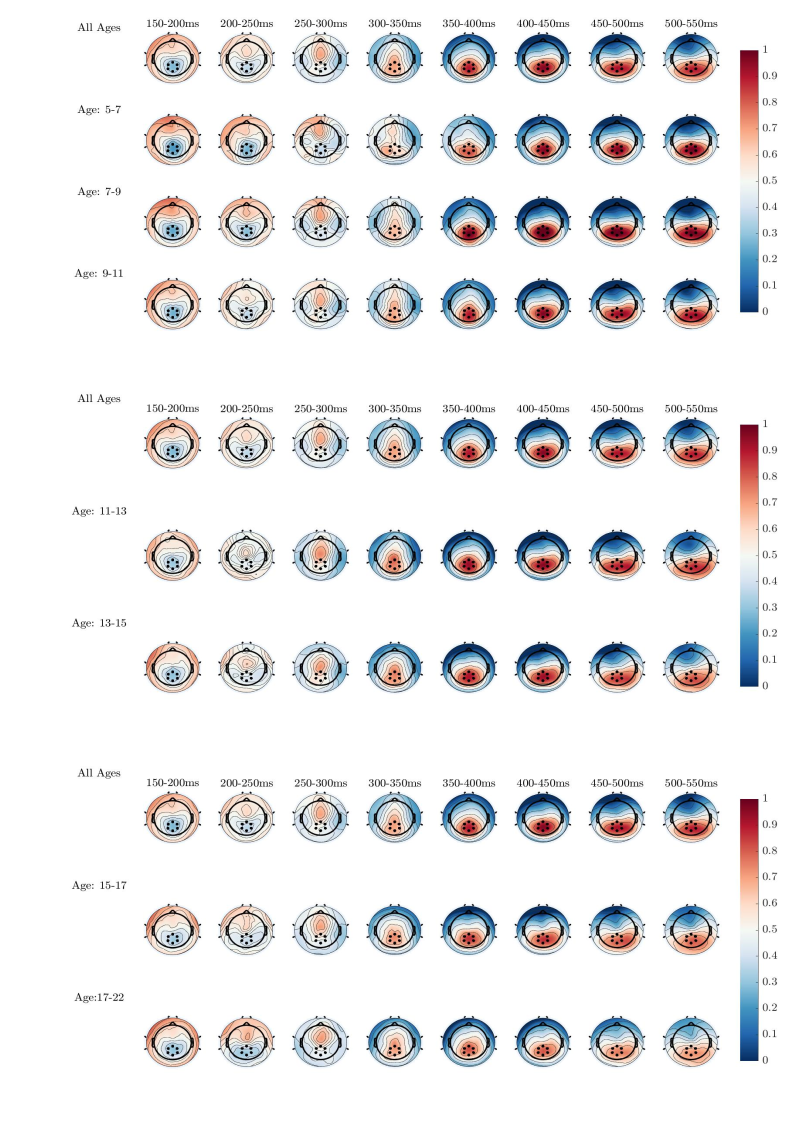
\includegraphics[width=0.8\linewidth]{Subfigures/topoall.png}
    \caption[]{Topoplots for Electrodes Selection.}
    \label{fig:elecsel}
\end{figure}

\newpage
\subsection*{Why Different Knowledge Index} \label{chap:stein}
Figure \ref{fig:steine} visualizes the study design in \textcite{steinemannTrackingNeuralCorrelates2016} paper. Since learning categories were created by comparing pre and posttest, the possibilty that a given stimulus location categorized as newly learned (i.e., pretest incorrect and posttest correct) could actually become known (i.e., twice correct) during the three sequence presentations led the authors to weight the newly learned learning categories with 0.5. In this thesis, behavior response is acquired after every sequence, therefore, the newly learned categories were not weighted. 
\begin{figure}[H]
\centering
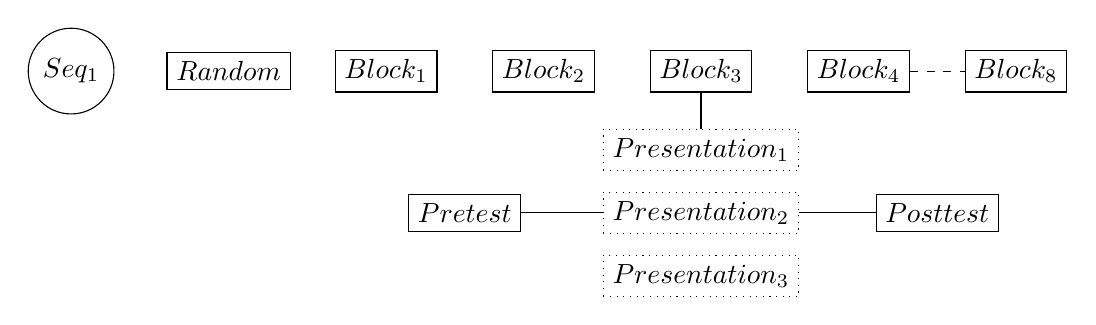
\begin{tikzpicture}
        \node at (0,0)[circle,draw] (c100)  {$Seq_1$};
        \node at (2,0) [rectangle,draw] (c200) {$Random$};
        \node at (4,0) [rectangle,draw] (c300) {$Block_1$};
        
         \node at (8,-2.6) [rectangle,draw,dotted] (c170) {$Presentation_3$};
        \node at (8,-1.8) [rectangle,draw,dotted] (c160) {$Presentation_2$};
         \node at (8,-1) [rectangle,draw,dotted] (c150) {$Presentation_1$};
        \node at (5,-1.8) [rectangle,draw] (c110) {$Pre test$};
        \node at (11,-1.8) [rectangle,draw] (c120) {$Post test$}; 
         \draw (c120)--(c160);
        \draw (c110)--(c160);

       \node at (6,0) [rectangle,draw] (c400) {$Block_2$};
        \node at (8,0) [rectangle,draw] (c500) {$Block_3$};
        \node at (10,0) [rectangle,draw] (c600) {$Block_4$};
       \node at (12,0) [rectangle,draw] (c700) {$Block_8$};
        \draw (c500)--(c150);
       \draw[dashed] (c600)--(c700);
      
    \end{tikzpicture}
\caption[]{Study design of experiement 2 in \textcite{steinemannTrackingNeuralCorrelates2016} visualized for the first sequence.} \label{fig:steine}
\end{figure}
\newpage
\subsection*{Network Analysis}
\begin{figure}[H]
    \centering
    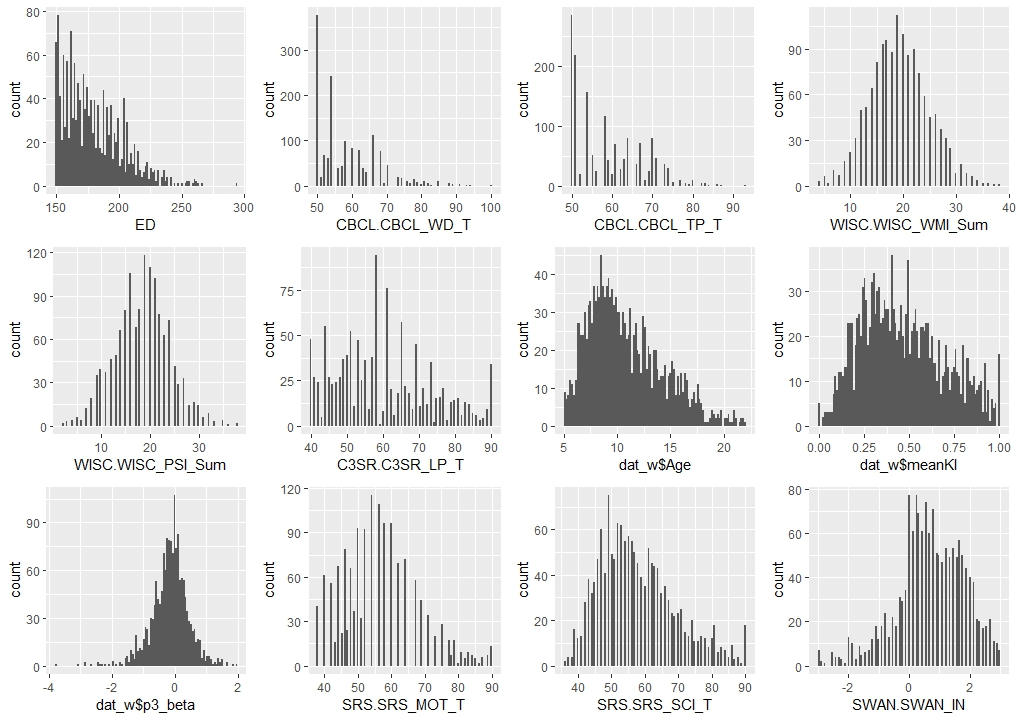
\includegraphics[width=0.8\linewidth]{Subfigures/Expl_dist_pre_trans.jpeg}
    \caption[]{Distribution of Variables included in the Network Analysis.}
    \label{fig:distall}
\end{figure}


\begin{figure}[H]
    \centering
    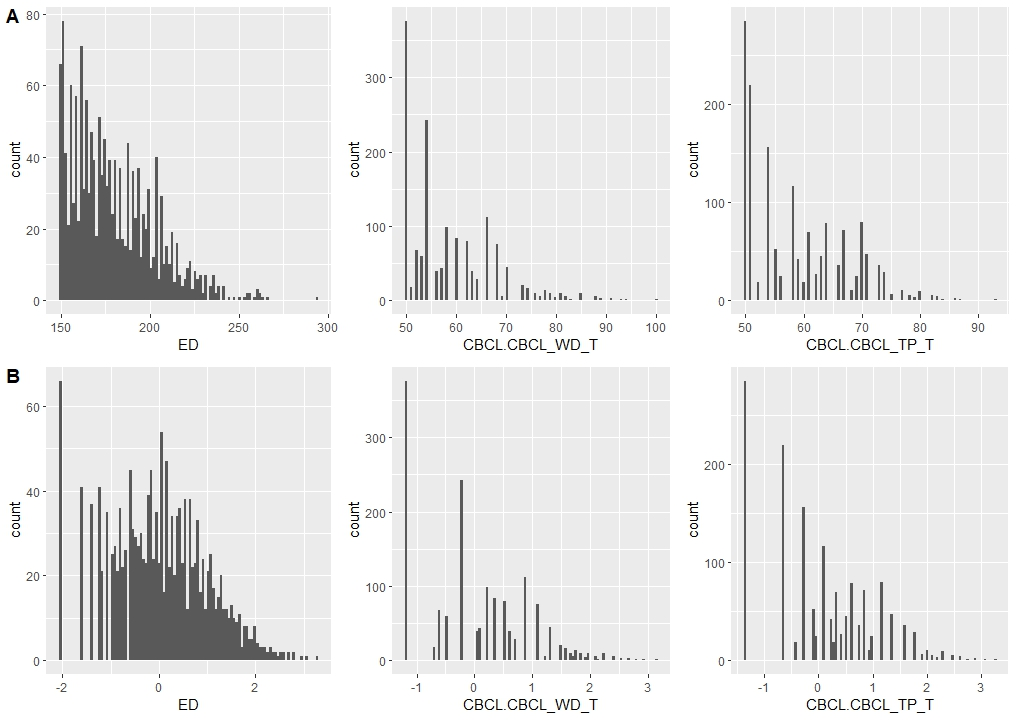
\includegraphics[width=0.6\linewidth]{Subfigures/Posttransform.jpeg}
    \caption[]{Distribution of Variables transformed. A: Before transformation. B: After transformation.}
    \label{fig:distaftert}
\end{figure}

\begin{table}[H]
\centering
\begin{tabular}{ccccccccccccc}
\hline
             & \textbf{V1} & \textbf{V2} & \textbf{V3} & \textbf{V4} & \textbf{V5} & \textbf{V6} & \textbf{V7} & \textbf{V8} & \textbf{V9} & \textbf{V10} & \textbf{V11} & \textbf{V12} \\ \hline
\textbf{V1}  &             &             &             &             &             &             &             &             &             &              &              &              \\
\textbf{V2}  & 0.30        &             &             &             &             &             &             &             &             &              &              &              \\
\textbf{V3}  & 0.48        & 0.09        &             &             &             &             &             &             &             &              &              &              \\
\textbf{V4}  & 0.08        & 0.00        & 0.00        &             &             &             &             &             &             &              &              &              \\
\textbf{V5}  & 0.00        & 0.00        & 0.00        & 0.35        &             &             &             &             &             &              &              &              \\
\textbf{V6}  & 0.00        & 0.00        & 0.00        & -0.25       & 0.00        &             &             &             &             &              &              &              \\
\textbf{V7}  & -0.18       & 0.17        & 0.10        & 0.00        & -0.19       & 0.00        &             &             &             &              &              &              \\
\textbf{V8}  & 0.00        & 0.00        & 0.00        & 0.23        & 0.18        & 0.00        & 0.21        &             &             &              &              &              \\
\textbf{V9}  & 0.00        & 0.00        & 0.00        & 0.07        & 0.00        & 0.00        & 0.00        & -0.07       &             &              &              &              \\
\textbf{V10} & 0.00        & 0.41        & -0.15       & 0.00        & 0.00        & 0.00        & 0.00        & 0.00        & 0.00        &              &              &              \\
\textbf{V11} & 0.14        & -0.08       & 0.23        & -0.09       & 0.00        & 0.00        & 0.00        & 0.00        & 0.00        & 0.00         &              &              \\
\textbf{V12} & 0.40        & -0.09       & -0.11       & 0.00        & -0.12       & 0.11        & 0.08        & -0.07       & 0.00        & 0.17         & 0.00         &              \\ \hline
\end{tabular}
\caption[]{Partical Correlation Matrix (estimated with ggmModSelect).}
\label{tab:parcorrm}
\end{table}

\begin{table}[]
\centering
\begin{tabular}{lllllllllllll}
\hline
\textbf{Nodes}                & \textbf{V1} & \textbf{V2} & \textbf{V3} & \textbf{V4} & \textbf{V5} & \textbf{V6} & \textbf{V7} & \textbf{V8} & \textbf{V9} & \textbf{V10} & \textbf{V11} & \textbf{V12} \\ \hline
\textbf{$R^2$} & 0.65        & 0.52        & 0.48        & 0.30        & 0.26        & 0.11        & 0.13        & 0.18        & 0.01        & 0.71         & 0.73         & 0.35         \\ \hline
\end{tabular}
\caption[]{Explained Variance of each Node in Network Analysis.}
\label{tab:Rsqu}
\end{table}







\newpage
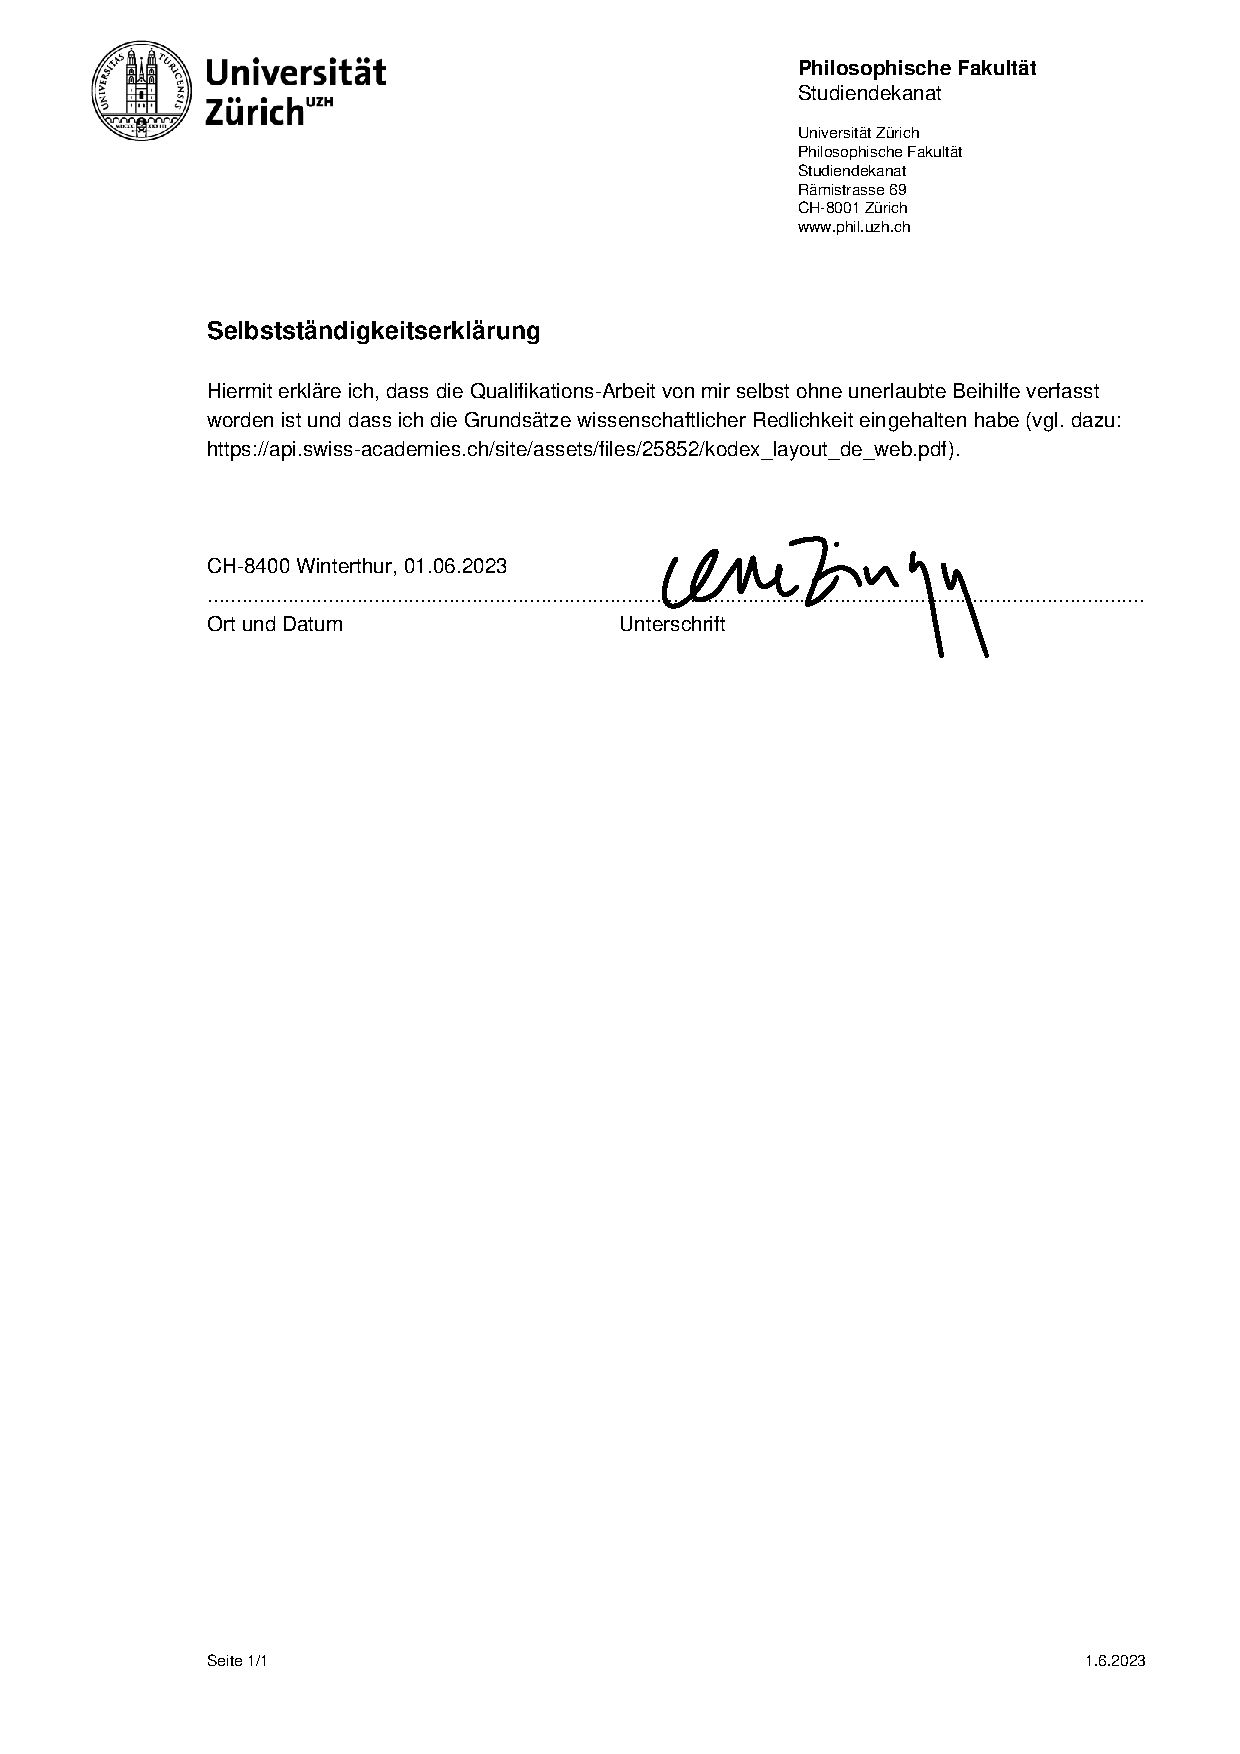
\includepdf[page=1]{Selbstständigkeitserklärung}
\end{document}